\documentclass[letterpaper,twocolumn,10pt]{article}
\usepackage{usenix,epsfig,endnotes}
\usepackage{amssymb}
\usepackage{amsthm}
\usepackage{enumitem}
\usepackage{tabularx}
\usepackage{boxedminipage}
\usepackage[override]{cmtt}
\usepackage[utf8]{inputenc}
\usepackage{color}
\usepackage{graphicx}
\usepackage{xspace}
\usepackage{amsmath,amstext,amssymb,amsfonts,latexsym}


\DeclareMathAlphabet{\mathcal}{OMS}{cmsy}{m}{n}

\newcommand{\kyle}[1]{\textcolor{blue}{[[\textsf{Kyle:  #1}]]}}
\newcommand{\fan}[1]{\textcolor{red}{[\textsf{Fan:  #1}]}}
\definecolor{darkgreen}{rgb}{0,0.6,0}
\newcommand{\ari}[1]{\textcolor{darkgreen}{[\textsf{Ari:  #1}]}}
\newcommand{\ethan}[1]{\textcolor{cyan}{[\textsf{Ethan: #1}]}}
\newcommand{\elaine}[1]{\textcolor{magenta}{[\textsf{elaine:  #1}]}}

\newtheorem{lemma}{Lemma}
\newtheorem{definition}{Definition}
\newtheorem{theorem}{Theorem}

%don't want date printed
\date{}

%make title bold and 14 pt font (Latex default is non-bold, 16 pt)
\title{Town Crier: \\ An Authenticated Data Feed for Smart Contracts}

%for single author (just remove % characters)
\author{
{\rm Your N.\ Here}\\
Your Institution
\and
{\rm Second Name}\\
Second Institution
\and
{\rm Name}\\
Name Institution
} % end author


%**** DEFINITIONS *********

\newcommand {\tcs} {Town Crier\xspace}
\newcommand {\tc} {TC\xspace}
\newcommand {\tcontract} {{TContract}\xspace}
\newcommand {\encname} {{Engine}\xspace}
\newcommand {\medname} {{Relay}\xspace}


\newcommand {\reqcont} {\ensuremath{{\cal C}_U}\xspace}
\newcommand {\tcont} {\ensuremath{{\cal C}_{TC}}\xspace}
\newcommand {\tcadd} {${\cal P}_{TC}$\xspace}
\newcommand {\sgxadd} {${\cal P}_{SGX}$\xspace}
\newcommand {\pkTC} {{\sf pk}_{TC}\xspace}
\newcommand {\skTC} {{{\sf sk}_{TC}}\xspace}

\newcommand {\dgreq} {{\sf req}\xspace}
\newcommand {\dgform} {{\sf params}\xspace}
\newcommand {\dgpay} {{\sf \$fee}\xspace}
\newcommand {\dg} {{\sf d}\xspace}
\newcommand {\dgret} {{\sf ans}\xspace}
\newcommand {\dgm} {{\sf data}\xspace}
\newcommand {\dgi} {{\sf d_{\mbox{$i$}}}\xspace}
\newcommand {\dgid} {{\sf id}\xspace}
\newcommand {\dgcallback} {{\sf callback}\xspace}

\newcommand {\att} {{\sf att}\xspace}

\newcommand{\fsgx}{\ensuremath{\mathcal{F}_{\textrm{sgx}}}\xspace}
\newcommand{\pk}{\ensuremath{{\sf pk}}}
\newcommand{\sk}{\ensuremath{{\sf sk}}}
\newcommand{\pkM}{\ensuremath{{\sf pk}_{\mathcal{M}}}}
\newcommand{\skM}{\ensuremath{{\sf sk}_{\mathcal{M}}}}
\newcommand{\pkU}{\ensuremath{{\sf pk}_{\mathcal{U}}}}
\newcommand{\pksgx}{\ensuremath{{\sf pk}_{\textrm{sgx}}}\xspace}
\newcommand{\sksgx}{\ensuremath{{\sf sk}_{\textrm{sgx}}}\xspace}
\newcommand{\pkurl}{\ensuremath{{\sf pk}_{\textrm{url}}}\xspace}
\newcommand{\rl}{\ensuremath{{\sf RL}}}
\newcommand{\relay}{\ensuremath{\mathcal{R}}}
\newcommand{\engine}{\ensuremath{\mathcal{E}}}
%\newcommand{\digest}{\ensuremath{{\sf digest}}}
\newcommand{\enclaveprog}{\ensuremath{{\sf prog}_{\textrm{encl}}}\xspace}
\newcommand{\sigatt}{\ensuremath{{\sigma_{\textrm{att}}}}}
\newcommand{\sigsgx}{\ensuremath{{\Sigma_{\textrm{sgx}}}}}
\newcommand{\weburl}{\ensuremath{{{\sf url}}}\xspace}
\newcommand{\clock}{\ensuremath{{{\sf clock}}}}
\newcommand{\algA}{\ensuremath{\mathcal{A}}}
\newcommand{\algB}{\ensuremath{\mathcal{B}}}

%*****************************

\begin{document}

\maketitle

% Use the following at camera-ready time to suppress page numbers.
% Comment it out when you first submit the paper for review.
% \thispagestyle{empty}

\subsection*{Abstract}
Smart contracts are programs that execute autonomously on blockchains. Many of their envisioned uses require them to consume data from outside the blockchain. (e.g., financial instruments rely on equity prices.) Trustworthy data feeds that can interface with smart contracts will thus be critical to any smart-contract system. 

	We present an authenticated data feed system called Town Crier (TC). TC builds on the observation that many web sites, such as major news and finance sites, already serve as trusted data sources for non-blockchain uses. TC acts as a bridge between such servers and smart contract systems, using trusted hardware to authenticate and scrape data from HTTPS-enabled websites and to generate authenticated, timestamped datagrams for relying smart contracts. It also includes a range of advanced features, such as private datagrams, which decrypt and evaluate ciphertext requests within TC's hardware.
	
	We describe the TC architecture, its underlying trust model, and its applications, and report on an implementation that uses the newly released SGX software development kit and furnishes data for the smart-contract system Ethereum. We will soon be launching TC as an online public service.
	

\section{Introduction}

Smart contracts are computer programs that autonomously execute the terms of a contract.
For decades they have been envisioned as a way to render legal agreements more precise, pervasive, and efficiently executable.
Szabo, who popularized the term ``smart contact'' in a seminal 1994 essay~\cite{szabosmartcontract94}, gave as an example a smart contract that enforces car loan payments. If the owner of the car fails to make a timely payment, a smart contract could programmatically revoke physical access and return control of the car to the bank. %The contract could additionally be programmed to do so only at a time that is safe for the the owner, e.g., while the car is parked.

Cryptocurrencies such as Bitcoin~\cite{bitcoin} provide key technical underpinnings for smart contracts: direct control of money by programs and fair, automated code execution through the decentralized consensus mechanisms underlying  blockchains. 
The recently launched Ethereum~\cite{yellowpaper,whitepaper} supports Turing-complete code and thus fully expressive, self-enforcing, decentralized smart contracts, a big step toward the vision of researchers and proponents.  
As Szabo's example shows, however, the most compelling applications of smart contracts---such as financial instruments---additionally require access to {\em data about real-world state and events}. 
%Similarly, financial contracts and derivatives, key applications for Ethereum~\cite{yellowpaper,whitepaper}, rely on data about financial markets such as equity prices. %Applications such as insurance policies are only realizable with data about weather, flights, delivery of goods, and so forth. 

\emph{Data feeds} (also known as ``oracles'') aim to meet this need. Very simply, data feeds are contracts on the blockchain that serve data requests by other contracts~\cite{whitepaper,yellowpaper}. A few data feeds exist for Ethereum today that source data from trustworthy websites, but provide no assurance of correctly relaying such data beyond the reputation of their operators (typically individuals or small entities). HTTPS connection to a trustworthy website would seem to offer a solution. Smart contracts, though, lack network access, and HTTPS does not digitally sign data for out-of-band verification. The lack of a substantive ecosystem of trustworthy data feeds is frequently cited as critical obstacle to the evolution of Ethereum and decentralized smart contracts 
in general~\cite{commblockstream}.

\paragraph{\bf Town Crier.} We introduce a system called \emph{Town Crier} (\tc) that addresses this challenge by providing an \emph{authenticated data feed} (ADF) for smart contracts. \tc acts as a high-trust bridge between existing HTTPS-enabled data websites and the Ethereum blockchain. It retrieves website data and serves it to relying contracts on the blockchain as concise pieces of data (e.g., stock quotes) called \emph{datagrams}. \tc uses a novel combination of Software Guard Extensions (SGX), Intel's recently released trusted hardware capability, and a smart-contract front end. It executes its core functionality as a trusted piece of code in an SGX \emph{enclave}, which protects against malicious processes and the OS and can \emph{attest} (prove) to a remote client that the client is interacting with a legitimate, SGX-backed instance of the \tc code. 

The smart-contract front end of \tcs responds to requests by contracts on the blockchain with attestations of the following form:

\vspace{-1ex}
\begin{itemize}[leftmargin=3mm]
  \item[] {``Datagram $X$ specified by parameters $\dgform$ is served by an HTTPS-enabled website $Y$ during a specified time frame $T$.''}
\end{itemize}
\vspace{-1ex}

\noindent A relying contract can verify the correctness of $X$ in such a datagram assuming trust only in the security of SGX, the (published) \tc code, and the validity of source data in the specified interval of time. 

Another critical barrier to smart contract adoption is the lack of {\em confidentiality} in today's ecosystems; all blockchain state is publicly visible, and existing data feeds publicly expose requests. \tc provides confidentiality by supporting {\em private} datagram requests, in which the parameters $\dgform$ are encrypted under a \tc public key for ingestion in \tc's SGX enclave and are therefore concealed on the blockchain. \tc also supports {\em custom} datagram requests, which securely access the online resources of requesters (e.g. online accounts) by ingesting encrypted user credentials, permitting \tc to securely retrieve access-controlled data.

We designed and implemented \tc as a complete, highly scalable, end-to-end system that offers formal security guarantees at the cryptographic protocol level. \tc runs on real, SGX-enabled host, as opposed to an emulator (e.g.~\cite{haven,VC3}). We plan to launch a version of \tc as an open-source, production service atop Ethereum, pending the near-future availability of the Intel Attestation Service (IAS), which is needed for use of SGX attestations. 

%In its initial form, \tcs will serve basic datagram requests to smart contract users essentially for free, requiring users only to defray the (small) cost of invoking \tc on the Ethereum blockchain. 

\paragraph{Technical challenges.} Smart contracts execute in an adversarial environment where parties can reap financial gains by subverting the contracts or services on which they rely. Formal security is thus vitally important. We adopt a rigorous approach to the design of \tcs by modeling it in the Universal Composibility (UC) framework, building on~\cite{hawk,sgxsok} to achieve an interesting formal model that spans a blockchain and trusted hardware. We formally define and prove that \tc achieves the basic property of datagram {\em authenticity}---informally that \tc faithfully relays current data from a target website. We additionally prove {\em fair expenditure} for an honest requester, informally that the fee paid by a user contract calling \tc is at most a small amount to cover the operating costs of the \tc service, even if the \tc host and other blockchain entities are malicious.
\ethan{Other blockchain entities? What is that referring to? Can we just remove that?}

Another contribution of our work is introducing and showing how to achieve two key security properties: {\em gas sustainability} and {\em TCB code minimization} within a new TCB model created by \tc's combination of a blockchain with SGX. 

Because of the high resource costs of decentralized code execution and risk of application-layer denial-of-service (DoS) attacks, Ethereum includes an accounting resource called {\em gas} to pay for execution costs.  Informally, {\em gas sustainability} means that an Ethereum service never runs of out of gas, a general and fundamental availability property. We give a formal definition of gas sustainability applicable to any Ethereum service, and prove that \tc satisfies it.

% offering a model for proving the property in other Ethereum services and one that may be extensible to other decentralized smart contract systems. 

We believe that the combination of blockchains with SGX introduced in our work will prove to be a powerful, general way to achieve confidentiality in smart contract systems and network them with off-chain systems. This new security paradigm, however, introduces a hybridized trusted computing base (TCB) that spans components with different trust models. We introduce techniques for using such a hybridized TCB securely while {\em minimizing the TCB code size}. In \tc, we show how to avoid constructing an authenticated channel from the blockchain to the enclave---bloating the enclave with an Ethereum client---by instead authenticating enclave outputs on the blockchain. We also show how to minimize on-chain signature-verification code. These techniques are general; they apply to any use of a similar hybridized TCB.

Other interesting smaller challenges arise in the design of \tc. One is deployment of TLS in an enclave. Enclaves lack networking capabilities, so TLS code must be carefully partitioned between the enclave and untrusted host environment. Another is hedging in \tc against the risk of compromise of a website or single SGX instance, which we accomplish with various modes of majority voting: among multiple websites offering the same piece of data (e.g. stock price) or among multiple SGX platforms.

\paragraph{Applications and performance.} 
%Today, smart contracts in Ethereum tend to be blockchain-bound, with little or no use of external data~\cite{}. 
We believe that \tc can spur deployment of a rich spectrum of smart contracts that are hard to realize in the existing Ethereum ecosystem. We explore three examples that demonstrate \tc's capabilities: (1) A financial derivative (cash-settled put option) that consumes stock ticker data; (2) A flight insurance contract that relies on private data requests about flight cancellations; and (3) A contract for sale of virtual goods and online games (via Steam Marketplace) for Ether, the Ethereum currency, using custom data requests to access user accounts. 

Our experiments with these three applications show that \tc is highly scalable. Running on just a single SGX host, \tc achieves throughputs of 15-65 tx/sec. \tc is easily parallelized across many hosts, as separate \tc hosts can serve requests with no interdependency. (For comparison, Ethereum handles less than 1 tx/sec today and recent work~\cite{blockchainscaling} suggests that Bitcoin can scale safely to no more 26 tx/sec with reparametrization.) For these same applications, experimental response times for datagram requests range from 192-1309 ms---much less than an Ethereum block interval (12 seconds on average). These results suggest that a few SGX-enabled hosts can support \tc data feed rates well beyond the global transaction rate of a modern decentralized blockchain.

\paragraph{\bf Contributions.}
We offer the following contributions:
\begin{itemize}[leftmargin=5mm]
\item
  \setlength{\itemsep}{2pt}
  \setlength{\parskip}{0pt}
  \setlength{\parsep}{0pt}
We introduce and report on an end-to-end implementation of \tcs, an authenticated data feed system that addresses critical barriers to the adoption of decentralized smart contracts. \tc combines a smart-contract front end in Ethereum and an SGX-based trusted hardware back end to: (1) Serve authenticated data to smart contracts without a trusted service operator and (2) Support {\em private} and {\em custom} data requests, enabling encrypted requests and secure use of access-controlled, off-chain data sources. We plan to launch a version of \tc soon as an open-source service.
\item We formally analyze the security of \tc within the Universal Composibility (UC) framework, defining functionalities to represent both on-chain and off-chain components. We formally define and prove the basic properties of datagram {\em authenticity} and {\em fair expenditure} as well as {\em gas sustainability}, a fundamental availability property for any Ethereum service. 
\item We introduce in \tc a hybridized TCB spanning the blockchain and an SGX enclave, a powerful new paradigm of trustworthy system composition. We present generic techniques that help shrink the TCB code size within this model as well as techniques to hedge against individual SGX platform compromises. 
\item We explore three \tc applications that show \tc's ability to support a rich range of services well beyond those in Ethereum today. Experiments with these applications also show that \tc can easily meet the latency and throughput requirements of modern decentralized blockchains. 

\end{itemize}

%\paragraph{\em Organization:} We present basic technical background for \tc (Section~\ref{sec:background}), followed by an architectural description (Section~\ref{sec:architecture}), a basic set of protocols (Section~\ref{sec:protocols}), the full, enhanced system protocols (Section~\ref{sec:enhanced_protocol}), and a formal security analysis (Section~\ref{sec:analysis}). We then present three example applications (Section~\ref{sec:applications}) which we use as the basis for performance evaluations of \tc (Section~\ref{sec:experiments}).  After presenting related work (Section~\ref{sec:related}), we conclude the paper (Section~\ref{sec:conclude}). The paper appendix includes implementation details, formal modeling and proofs, and future directions omitted from the paper body.





\section{Background}
\label{sec:background}

In this section, we provide basic background respectively on the main technologies \tc incorporates, namely SGX, TLS / HTTPS, and smart contracts.

\subsection{SGX}
Intel's Software Guard Extensions (SGX) is a set of new instructions that confer hardware protections on user-level code. Its goal is to provide \emph{isolated execution}. SGX enables a process to execute in a protected address space known as an {\em enclave}. It protects the confidentiality and integrity of a process in an enclave from other software on the same host, including the operating system, as well as from certain forms of hardware attack, such as memory probes. 

A enclave process cannot make system calls, nor can it execute code outside the enclave region. As a means of communicating with processes outside the enclave, however, it can read and write memory outside the enclave region, consistent with OS setting of page permissions. Thus  isolated execution in SGX may be viewed in terms of an ideal model in which a process is guaranteed to execute correctly and with perfect confidentiality, but relies on a (potentially malicious) operating system for network and file-system access.\footnote{This model is a simplification, as SGX is known to expose some of the internal state of an enclave to the operating system (e.g., making page faults or cache timings visible to the exception handler~\cite{sgxexplained}), creating potential side-channel vulnerabilities. We regard side channels as outside the scope of this paper, and thus assume an ideal model of isolated execution.}

Another feature of SGX is its support for \emph{attestation}, which allows a remote system to verify the software in an enclave and communicate securely with it. When an enclave is created, the CPU produces a hash of its initial state known as a {\em measurement}. The software in the enclave may at a later time request a report, which includes a measurement and any supplementary data provided by the process, such as a public key and timestamp. The report may be digitally signed (by a trusted process called a ``quoting enclave'') using a hardware-protected key to produce a proof that the measured software is running in an SGX-protected enclave. This proof, known as a {\em quote}, may be verified by a remote system, while the associated public key in the supplementary data can then be used by the remote system to establish a secure channel with the enclave or verify signed data it emits. We use the generic term {\em attestation} to refer to a quote, and denote it by \att. We assume that a trustworthy measurement of the code for the enclave component of \tc is available to any client that wishes to verify an attestation. SGX signs quotes using a \emph{group signature} scheme called EPID~\cite{}. This choice of primitive is significant in our design of \tcs, as EPID is a proprietary signature scheme and is not supported in Ethereum.

SGX additionally provides a trusted time source via the function \texttt{sgx\_get\_trusted\_time}.~On invoking this function, an enclave obtains a measure of time relative to a reference point labeled with a nonce. We refer to this as the \emph{clock reference point}. It remains stable for a given nonce, but SGX does not provide a source of absolute or wall-clock time, a limitation that we must work around in \tc.

\subsection{HTTPS / TLS}

We assume basic familiarity by readers with TLS and HTTPS (HTTP over TLS). As we explain later, an important feature of HTTPS that we employ in \tc is its amenability to partitioning into interoperable layers: an HTTP layer interacting with web servers, a TLS layer handling handshakes and secure communication, and a TCP layer providing reliable data stream. \tc places the HTTP layer and TLS layer in an enclave, enabling code in the enclave to establish a secure channel with a remote server, with only the TCP layer controlled by untrusted code outside the enclave. 


\subsection{Smart contracts}

Smart contracts are the expression of contractual agreements, including financial instruments, as executable code. In the context of cryptocurrencies, the term refers specifically to autonomously executing scripts that reside on a blockchain and can manipulate and control currency. Bitcoin has a scripting language that can serve to implement a limited form of smart contract, but it is not Turing-complete and lacks support for loops. 

Ethereum is the first decentralized blockchain with a Turing-complete scripting language and thus full support for smart contracts. Other Turing-complete smart contract systems exist, such as Counterparty~\cite{}, which runs as a Bitcoin overlay, but is not fully decentralized. Ethereum has its own associated cryptocurrency called \emph{ether}. (At the time of writing, 1 ether has a market value of a little more than \$2 U.S. \ethan{I believe this is off by an order of magnitude, I think 10 ether is about \$2}) While \tc can be adapted in principle to any smart contract system, we report on an implementation directed at Ethereum.

A smart contract in Ethereum is represented as what is called a \emph{contract account}, endowed with code, a currency balance, and persistent memory in the form of a key/value store. Contract code executes in response to receipt of a \emph{message} from another contract or a \emph{transaction} from a non-contract (\emph{externally owned}) account, informally what we call a ``wallet.'' Thus, contract execution is always initiated by a transaction. Informally, a contract only executes when ``poked,'' and poking progresses through a sequence of entry points until no further message passing occurs (or until there is a shortfall in gas, as explained below). Transactions in Ethereum are digitally signed for a wallet using ECDSA on the curve Secp256k1 and the hash function SHA3-256. \ethan{should we cite the yellow paper here?}

A smart contract accepts messages as inputs to any of a number of designated functions. These entry points are determined by the contract creator and represent the API of the contract. Once created, a contract executes autonomously; it persists indefinitely, with even its creator unable to modify its code. (There's one exception: a special opcode \texttt{suicide} will wipe code from a contract account.) As a simple abstraction, then, a smart contract may be viewed as an {\em autonomous agent} on the blockchain. \ethan{I'm concerned that this makes it sound like contracts can be self-activating. Someone needs to call a function explicitly for them to do anything.} 

To prevent Denial-of-Service (DoS) attacks, inadvertent infinite looping within contracts, and generally to control resource expenditure by the network,
Ethereum implements uses a resource called \emph{gas} to power contracts.
Every operation, including sending data to a transaction, executing computation, and storing data, has a fixed gas cost.
Transactions and messages include a parameter (\texttt{GASLIMIT}) specifying a bound on the amount of gas expended by the computations they initiate.
When a function call is made, the child function expends gas from the same source as the parent function.
Should a function fail to complete due to a shortfall in gas,
it is aborted and any state changes induced by the partial computation are rolled back to their pre-call state;
previous computations along the call path, however, are retained.

Along with the \texttt{GASLIMIT} parameter, a \texttt{GASPRICE} parameter is included that specifies the maximum amount in ether that the transaction is willing to pay per unit of gas. The transaction thus succeeds only if the initiating account has a balance of \texttt{GASLIMIT} $\times$ \texttt{GASPRICE} ether and \texttt{GASPRICE} is high enough to be accepted by the system (miner). 

The management of gas, as we show in our design of \tcs can be delicate. Without careful construction, for example, the smart contracts representing \tc's interface on the Ethereum blockchain can be caused by an attacker to exhaust the ether used to power the delivery of datagrams. 





\section{Architectural Overview: Basic TC System}

The blockchain interface to \tc is the smart contract \tcont. \tcont is designed to present a simple API to a relying contract / requester \reqcont. \reqcont sends to \tcont a specification of the datagram it is requesting, along with payment. The datagram specification includes the data being sought and may also include parameters, such as the time at which the data should be retrieved, the target source or sources, and so forth. \tcont simply returns the requested data to \reqcont. The interaction between \reqcont and \tcont takes place entirely on the blockchain.

The complexity of \tc resides primarily in its backend, which must monitor, keep track of, and fulfill datagram requests passing from requesters through \tcont. Additionally, to validate the trustworthiness of \tc, the entity or entities creating \reqcont must verify a hardware- (SGX-)generated attestation. So \tc must also support a service to fulfill attestation requests off-chain. 

\subsection{Architecture}

The \tcs system includes three main components: The \tcontract, the \encname, and the \medname. The \encname and \medname reside on the \tc server, while the \tcontract resides on the blockchain. An architectural schematic showing the roles of these components is given in Figure~\ref{fig:overview}.

\vspace{-2mm}
\begin{figure}[h!]
\centering
\includegraphics[width=\columnwidth]{figures/OverviewFig}
\caption{{\bf Basic Town Crier architecture.}}
\label{fig:overview}
\end{figure}
\vspace{-2mm}

\paragraph{The \tcontract (\tcont).} The \tcontract (denoted by \tcont) is a smart contract that acts as the blockchain front-end of the \tc service, and thus an interface between relying contracts and \tc. It accepts datagram requests from a requester \reqcont and returns corresponding datagrams from \tc. Additionally, the \tcontract manages \tc monetary resources, which in Ethereum take the form of ether (money) and gas (``fuel'' for contracts). 

\paragraph{The \encname.}
The \encname ingests and fulfills datagram requests from the blockchain. To obtain the data for inclusion in datagrams, it queries external data sources, specifically HTTPS-enabled internet services. It returns a datagram to a requesting contract \reqcont as a digitally signed blockchain message. The \encname runs in an SGX enclave, and is thus secured against an adversarial OS as well as other process on the host. 

\paragraph{The \medname.} As an enclave process, the \encname lacks direct network access. Thus the \medname handles bidirectional network traffic on behalf of the \encname. Specifically, the \medname provides network connectivity from the \encname to three different types of entities: 

\begin{enumerate}
\item {\em The Blockchain (the Ethereum system):}  The \medname scrapes the blockchain in order to monitor the state of the \tcontract  \tcont. In this way, it performs implicit message passing from \tcont to the \encname, as neither component itself has network connectivity. Additionally, the \medname places messages emitted from the \encname (datagrams) on the blockchain.
\item {\em Clients:} The \medname runs a web server to handle off-chain service requests from clients, specifically, requests for attestations from the \encname. As we soon explain, an attestation provides a unique public key for the \encname instance to the  client and proves that the \encname is executing correct code in an enclave and that its clock is correct in terms of absolute (wall-clock time). A client that successfully verifies an attestation can then safely create a relying contract \reqcont that uses the \tc.
\item {\em Data sources:} The \medname relays traffic to and from data sources (HTTPS-enabled servers) queried by \encname. 
\end{enumerate}

The \medname is an ordinary user-space application. It does not benefit from integrity protection by trusted hardware and thus, unlike the \encname, can be subverted by an adversarial OS on the \tc server, causing network delays or failures. As we explain in detail later in the paper, however, a key design aim of \tc is that \medname should be unable to cause incorrect datagrams to be produced or users to lose money. In general, the \medname~{\em can only mount denial-of-service attacks against \tc}. 

\paragraph{End-to-end datagram processing.}
In summary, then, a datagram request is initiated by a requester \reqcont. \reqcont sends a datagram request to \tcont on the blockchain. Using network services provided by the \medname, the \encname obtains the request from the blockchain. It contacts a data source to obtain the requested data and composes a datagram, which it sends back to \reqcont.

As a simple example, \reqcont might request a stock ticker  (e.g., the price of IBM at 3 p.m. on 15 Jan 2017). The \encname would fetch the requested data from an online service (e.g., https://www.google.com/finance) and place it in a datagram for transmission via \tcont to \reqcont.

%In addition to servicing datagram requests, the \encname may be queried by a client to provide an off-chain, hardware-backed attestation $\att$ on the state of the \encname---both its executing code and its clock. It is to support this service that \medname includes a web server. We do not depict this service in Figure~\ref{fig:overview}, and defer its discussion to later in the paper.

We now make this data flow more precise. 

\subsection{Datagram processing: Data flow}

We denote a datagram instance, namely the set of message values associated with a datagram request, by $\dgi$, where $i$ is a unique instance index. (We explain in Section~\ref{sec:implementation} how this index is computed.) 

A datagram request by \reqcont takes the form of a message $\dgi.\dgreq$ to \tcont on the blockchain. This message $\dgi.\dgreq = (\dgi.\dgform, \dgi.\dgpay)$ includes both a specification $\dgi.\dgform$ of the requested datagram (e.g., a stock ticker and desired time) and a payment $\dgi.\dgpay$, which in Ethereum may include gas to cover the execution cost of the request as well as a service fee. \tcont receives a return message $\dgi.\dgret = (\dgi.\dgform, \dgi.\dgm)$ from the $\tc$ service where $\dgm$ contains the data (e.g., the desired stock ticker price). \tcont checks the consistency of $\dgi.\dgform$ on the incoming and outgoing messages, and if they match forwards $\dgi.\dgm$ to \reqcont. Where clear from context, we omit the prefix $\dgi$ from our notation.

Figure~\ref{fig:dataflow} shows the data flows involved in processing a datagram request. For simplicity, the figure omits the \medname, which is only responsible for data passing.


\begin{figure}[h!]
\centering
\includegraphics[width=\columnwidth]{figures/DataflowFig}
\caption{{\bf Data flows in datagram processing.}}
\label{fig:dataflow}
\end{figure}


Digital signatures are needed to authenticated messages, such as $\dgret$, entering the blockchain from an external source. We let $(\skTC, \pkTC)$ denote the private / public keypair associated with the \encname for such message authentication. For simplicity, we assume for the time that the \encname can send signed messages directly to \tcont. Later we explain how Ethereum requires a slightly different approach.

\subsection{Security model}

Here we given an overview of our security model for \tc, providing more details in our security analysis in section~\ref{}. We assume the following:

\begin{itemize}
\item {\em \encname security:} Leveraging the basic properties of SGX, an attestation $\att$ proves to a verifier (client) about an \encname instance that: (1) The instance is executing correct code, i.e., behaves honestly; (2) For a public key $\pkTC$ included in the attestation, the corresponding private key $\skTC$ is known only to the instance; and (3) The SGX / enclave clock is set to absolute (wall-clock) time $T$ asserted in $\att$, where $T$ is verifiable by a client (requesting a fresh attestation) to within accuracy $\Delta$ (e.g., 100ms).

\item {\em Network communication:} The \medname (and other untrusted components of the \tc server) can tamper with or delay communications to and from the \encname, but cannot otherwise observe or alter the behavior of the \encname. Thus the \medname is simply subsumed by an adversary that controls the network. 

\item {\em Blockchain communication:} Message sources are authenticable, i.e., the originating blockchain address of a message can be correctly identified, and messages are integrity protected, but not confidential. This includes messages sent from the \encname, whose public key $\pkTC$ is bound in \tc to a blockchain account. 
\end{itemize}

\subsection{Design rationale: Role of \tcont}

One could imagine an alternative strawman protocol such as the following...

It is perhaps not immediately evident why our architecture makes use of the contract \tcont to intermediate between \reqcont and the \encname. In principle the \tc service could scrape the blockchain, identify contracts with state explicitly indicating a request for datagrams and send them datagrams and accompanying attestations directly.  This would result in a conceptually simpler protocol, eliminate some in-blockchain message passing, and also ensure that \reqcont consumes only fresh SGX attestations. In contrast, in our design, it is most practical for users to verify an SGX attestation offline at the time \reqcont is created, raising the risk that the attestation goes stale. (Of course, revocation must be handled in either case.)

The rationale for this design choice is twofold: First, \tcont manages the payment of fees (ether and gas) for the \tc service, creating a fair exchange of datagrams for fees. Second, although \reqcont could in principle verify a TC attestation directly, in practice, this would not be practical today. In Ethereum, opcodes for in-contract cryptographic operations are very limited and do not currently support public-key cryptography. (Digital signatures are supported only for messages from non-contract accounts.) 













\section{\tc Protocol}

We now describe the operation of \tc at the protocol level. The basic protocol is conceptually simple: A user contract \reqcont requests a datagram from the \tcontract \tcont. \tcont forwards the request to \engine and then returns the request to \reqcont. There are many details, however, relating to message contents and protection and the need to connect the off-chain parts of \tc with the blockchain.

First, we give a brief protocol overview. Then we enumerate the data flows in \tc. Finally, we provide a component-level view of the protocol by specifying the functionalities embodied in the \tcontract, \medname, and \encname. We present these  as ideal functionalities, inspired by the universal-composability (UC) framework, in order to abstract away implementation details and as a springboard for formal proofs of security. We omit details in this section on how payment is incorporated into \tc; this delicate aspect of the system design is deferred to Section~\ref{}.

\subsection{Datagram lifecycle}

The lifecycle of a datagram may be briefly summarized in the following steps:

\begin{itemize}
\item {\bf Initiate request.} \reqcont sends a datagram request to \tcont on the blockchain.

\item {\bf Monitor and relay.} The \medname monitors \tcont and relays any incoming datagram request with parameters \dgform to the \encname.

\item {\bf Securely fetch feed.} To process the request specified in \dgform, the \encname contacts a data source via HTTPS and obtains the requested datagram. It forwards the datagram via the Relay to \tcont.

\item {\bf Return datagram.} \tcont returns the datagram to \reqcont.
\end{itemize}

We now make this data flow more precise. 

\subsection{Data flows}

A datagram request by \reqcont takes the form of a message $m_1 = (\dgid, \dgcallback, \dgform)$ to \tcont on the blockchain. Here, $\dgid$ is a unique request identifier (which we explain later how to compute in practice); $\dgcallback$ specifies the entry point in \reqcont to which the datagram is to be returned. (In principle, $\dgcallback$ could specify an entry point in a different contract, but \tc does not yet adopt this generalization. $\dgform$ specifies the requested datagram, e.g., ${\sf params} := (\weburl, {\sf spec}, T)$, where $\weburl$ is the target data source and {\sf spec} specifies content of a the datagram to be retrieved (e.g., a stock ticker at a particular time), while $T$ specifies the delivery time for the datagram. 

\tcont forwards $m_2 = (\dgid, \dgform)$ to the \encname. It receives in return a return message $m_3 = (\dgid, \dgform, \dgm)$ from the $\tc$ service, where $\dgm$ is the datagram, i.e., contains the data (e.g., the desired stock ticker price). \tcont checks the consistency of $\dgform$ on the incoming and outgoing messages, and if they match forwards $\dgm$ to the entry point \dgcallback in \reqcont in message $m_4$. 

Fig.~\ref{fig:dataflow} shows the data flows involved in processing a datagram request. For simplicity, the figure omits the \medname, which is only responsible for data passing.


\begin{figure}[h!]
\centering
\includegraphics[width=\columnwidth]{figures/DataflowFig}
\caption{{\bf Data flows in datagram processing.}}
\label{fig:dataflow}
\end{figure}


Digital signatures are needed to authenticated messages, such as $\dgret$, entering the blockchain from an external source. We let $(\skTC, \pkTC)$ denote the private / public keypair associated with the \encname for such message authentication. For simplicity, Fig.~\ref{fig:dataflow} assumes that the Engine can send signed messages directly to \tcont. We explain shortly how Ethereum requires a slightly different approach in which \tc sends messages via an Ethereum wallet \tcadd.


\subsection{Use of SGX.}
Our protocols in \tc rely on the ability of SGX attestation to bind an instance of the \encname to a public key and for the \encname to maintain accurate absolute or wall-clock time. To simplify our presentation, we defer most details of our formal model of SGX capabilities and specification of protocols for attestation generation to the paper appendix. Instead, we first explain and present a simple abstraction of these capabilities suitable for our \tc protocol descriptions. 

Let $\enclaveprog$ represent the code for \encname, which we presume is trusted by all system participants. To avoid having to verify an EPID group signature on the blockchain, we have clients obtain SGX attestations from the \medname and verify them off-chain. As noted above, it is possible to bind an enclave process instance running \enclaveprog to a key pair $(\pkTC, \skTC)$ by including the public key pair in an attestation. We take this approach in \tc. 

\paragraph{Binding $\enclaveprog$ to Ethereum wallet \tcadd.}
Information can only be inserted into the blockchain in Ethereum as a transaction from a wallet. Thus, the only way the \medname can relay messages form the \encname to \tcont is through a wallet (again, formally, an externally owned account) \tcadd. Since the \medname may corrupt messages, however, it is critical that they be authenticated by the \encname. Since Ethereum itself 
already verifies signatures on transactions from externally owned accounts (i.e., users interact with the  Ethereum blockchain through an authenticated channel), \tc uses a trick to {\it piggyback verification of enclave signatures on top of Ethereum's already existing transaction signature verification mechanism}. 

Very simply, the \encname creates \tcadd with the public key \pkTC. 

To make this idea work fully, the public key $\pkTC$ must be hardcoded into \tcont. A client creating or relying on a contract that uses \tcont is responsible for making sure that this hardcoded $\pkTC$ has an appropriate SGX attestation before interacting with the $\tcont$  blockchain contract.  Let {\sf Verify} denote a verification algorithm for EPID signatures. Fig.~\ref{fig:att_check} gives the protocol for a client to check that \tcont is backed by a valid \encname instance. This protocol does not include a mechanism for \emph{revocation} of a compromised SGX instance, an issue we discuss later in the paper.

In summary, then, we may assume in our protocol specifications that {\em all relying clients have verified an attestation for \encname and thus that datagram responses passed from \tcadd to \tcont are trusted to originate from \engine.} 


\paragraph{\bf Clock.}
Additionally, as noted above, trusted clock provides only relative time with  respect to a reference point, not absolute time. Thus, when initialized, the \encname is provided with the current wall-clock time by a trusted source, e.g., the \medname (under a trust-on-first-use model). The SGX attestation generated by the \encname includes the current wall-clock time, which clients may verify in real time. Thus, a client can determine the absolute clock time of \encname to within a high degree of accuracy, bounded by the round-trip time of its attestation request plus the attestation verification time--on the order of hundreds of milliseconds in a wide-area network~\cite{}. A high degree of accuracy is potentially useful for some applications but sub-second accuracy is not required for most. Ethereum has a block interval of 12s and the clock serves in \tc primarily to: (1) Schedule connections to data sources and (2) To check TLS certificates for expiration when establishing HTTPS connections.
\ari{Let's give the attestation API a function name.} We present a formal model and protocol specification in the paper appendix.


\paragraph{\bf Notation.} We model execution in SGX in terms of a functionality $\fsgx$ operating in a stateful manner on \enclaveprog. This functionality may be be invokes through transmission of one of three messages to \enclaveprog: \initcall, which creates the enclave with \enclaveprog as its initial state and triggers measurement quotes, \attcall, which causes \engine to initiate an attestation with the public key and current time as supplementary data, and (\resumecall, $X$) which initiates an execution of \enclaveprog on a fresh input $X$. (We assume that \enclaveprog exits only when it completes processing of a given input.) We let $\fsgx[\enclaveprog, \relay]$ denote invocation of $\fsgx$ on \enclaveprog by \relay. We let $\clock()$ denote measurement of the SGX clock from within the enclave; $\clock()$ returns the current wall-clock time (in a canonical format such as seconds since the Unix epoch January 1, 1970 00:00 UTC).\ari{What format do we actually use?}

We abstract away the use of group signatures in EPID and simply denote the keypair associated with an SGX instance in \tc by $(\pkM, \skM)$. We let $\Sigma.{\sf Sign}({\sk}, X)$ denote a digital signature under private key $\sk$ of message $X$, and $\Sigma.{\sf Verify}({\sk}, \sigma, X)$ denote the corresponding verification operation.

\begin{figure}[htb!]
\begin{boxedminipage}{\columnwidth}
\begin{center}
{\bf User: offline attestation of SGX enclave}
\end{center}
\begin{tabular}{l}
{\bf Inputs}: $\pkM$, $\pkTC$, $\enclaveprog$, $\sigatt$ \\[5pt]
{\bf Checks:} \\
Assert $\enclaveprog$ is the expected enclave code\\
Assert $\sigsgx.{\sf Verify}(\pkM, \sigatt, (\enclaveprog, \pkTC))$ \\
Assert \tcont is correct and parametrized w/ \pkTC\\
{\it //~now okay to rely on \tcont}
\end{tabular}
\end{boxedminipage}
\caption{A client checks an SGX attestation on the enclave's code $\enclaveprog$ and public key $\pkTC$; the client
checks that $\pkTC$ is hardcoded into \tc blockchain contract \tcont before 
using \tcont.
} 
\label{fig:att_check}
\end{figure}


\begin{figure}
\begin{boxedminipage}{\columnwidth}
\begin{center}
{\bf $\fsgx[\enclaveprog, \relay]$: abstraction for SGX}
\end{center}
\begin{tabular}{l}
{\bf Hardcoded:} $\skM$ \\[5pt]

{\bf Assume:} \\ 
$\enclaveprog$ has entry points {\bf Initialize} and {\bf Resume}\\[5pt]

{\bf Initialize:}\\
On receive ``initialize'' from $\relay$: \\
\quad Let ${\sf outp} := \enclaveprog.{\bf Initalize}()$  \\
\quad $\sigatt := \sigsgx.{\sf Sign}(\skM, (\enclaveprog, {\sf outp}))$ \\[-1pt]
\qquad \qquad {\it //~models group sig.}\\
\quad Output  $({\sf outp}, \sigatt)$\\[5pt]

On receive (``resume'', ${\sf params}$) from $\relay$: \\
\quad Let ${\sf outp} := \enclaveprog.{\bf Resume}({\sf params})$  \\
\quad Output ${\sf outp}$ 
\end{tabular}
\end{boxedminipage}
\caption{Formal abstraction for SGX attested execution. 
We adopt a similar modeling approach by Shi et al., where
the SGX group signature is abstracted with a normal signature
by a manufacturer key $\pkM$. 
\elaine{cite our sok paper}
The above functionality only models a subset of SGX features
that is sufficient for our formalism.
}
\end{figure}


\paragraph{Formally abstracting SGX.}
\elaine{refer to figure and explain}



\subsection{A payment-free basic protocol}
For simplicity, we first specify functionalities in a payment-free version of our basic protocol, i.e., one that does not include gas or fees. Later, in our implementation discussion, we explain how we handle these two forms of payment, and we prove payment-related properties in the paper appendix. For simplicity, we assume a single instance of \engine and a since \tc server, although our architecture could scale up to multiple instances of either. To show messages corresponding to those in Fig.~\ref{fig:dataflow}, we use the label ({\bf msg.}~$m_i$)

\paragraph{The \tcontract \tcont.} The \tcontract, as noted above, accepts a datagram request $(\dgid, \dgform, \dgcallback)$, forwards it to the \tc server, and sends the resulting datagram $\dgm$ to the entry point \dgcallback in the requesting contract \reqcont. As we explain in Section~\ref{sec:implementation}, the blockchain verifies that the response is correctly signed under $\engine$'s key $\pkTC$, so \tcont need not verify the signature explicitly. \tc does, however, have a subtle security requirement. Specifically,  for a given datagram request $\dgid$, \tcont verifies that $\dgform' = \dgform$, where $\dgform$ is the digitally signed message produced by \engine and $\dgform$ is the locally stored parameters. The check is necessary to prevent \relay from corrupting datagram requests passed by \tcont (which, as a public function, has no means of digitally signing requests). \tcont is specified in Fig.~\ref{tbl:tc-contract}. As a reminder, we assume (and enforce) the condition that $\dgid$ is unique to a given request.

\begin{figure}[!htb]
\begin{tabularx}{\linewidth}{|@{\hspace{3pt}}r@{\hspace{1ex}}X@{\hspace{3pt}}|}
  \hline

  \multicolumn{2}{|c|}{{\bf Program for Town Crier blockchain contract \tcont}} \\ [1ex]
  {\bf Request:} & On recv $(\dgid, \dgform, \dgcallback)$ from some $\reqcont$:   
\\
& \qquad \qquad \qquad \qquad \qquad \qquad {\sgray{\it //~{\bf msg.}~$m_1$}} \\
%                 & If $(\${\sf fee} < F_{\rm min}$ or $\${\sf fee} > F_{\rm max})$ \\
%                 & \hspace*{1em} Return $\${\sf fee}$ to $\pkU$ \\
                 & Record $(\dgid, \dgform, \dgcallback)$ \\[5pt] 
%		 & Send $(\dgid, \dgform)$ to \relay \\
%\multicolumn{2}{|c|}{\sgray {\it // above implemented by \relay monitoring the blockchain}}\\[5pt]
  {\bf Deliver:} & On recv $(\dgid, \dgform, \dgm)$ from $\tcadd$: \\
		 & Let $(\dgid, \dgform', \dgcallback)$ be a most recently recorded tuple corresponding to $\dgid$ :\\
		 & Assert $\dgform = \dgform'$\\
                 & Call ${\dgcallback}({\dgm})$ \quad \sgray{\it //~{\bf msg.}~$m_4$}\\
%                 & Send $\${\sf fee}$ ether to $\Psgx$. \\

  \hline
\end{tabularx}
\caption{
The Town Crier \tcontract \tcont.
}
\label{tbl:tc-contract}
\end{figure}

\paragraph{The \encname \engine.} When initialized through an \initcall call, \engine sets its absolute clock (by setting a reference point) and generates a keypair $(\pkTC,\skTC)$ to which it binds by placing $\pkTC$ in attestation requests. Given input \resumecall $({\sf id}, {\sf params})$, \engine contacts the requested data source via HTTPS and checks that the corresponding certificate {\sf cert} is valid, i.e., not expired. We defer discussion of certificate revocation to Section~\ref{}. \engine then fetches the requested datagram and returns it to \relay along with the inputs, all digitally signed. The protocol for \engine is shown in Fig.~\ref{fig:engineprot}.

\begin{figure}[!h]
\begin{boxedminipage}{\columnwidth}
\begin{center}
{\bf Program for \tcs~\encname \engine (enclave)}
\end{center}
\begin{tabular}{l}
%{\bf Inputs}:  ${\sf params}$, \\[5pt]
%{\bf Initialize}:  On recv (\initcall, $T_0)$: \\ %{\it //~called only once upfront}\\
{\bf Initialize}:  On recv (\initcall): \\ %{\it //~called only once upfront}\\
%\quad Set clock reference point\\
%\quad Record $T_0$ \elaine{this is never used} \\ 
%\elaine{i deleted the clock implementation, we can separate abstraction from implementation.}\\
\quad $(\pkTC, \skTC) := \Sigma.{\sf KeyGen}(1^\lambda)$\\
%\quad Record $(\pkTC, \skTC)$\\
\quad Output $\pkTC$   \\
\sgray{\it/*$\fsgx$ attests to the code and the output $\pkTC$,} \\
\quad \sgray{see Figure \elaine{refer}*/}
\\[3pt]

%{\bf Attest}:  On recv \attcall: \\ %{\it //~called only once upfront}\\
%\quad $T := \clock()$\\
%\quad Call quoting enclave with supp.~data $(\pkTC, T)$
%\\[5pt]

{\bf Resume:} On recv (\resumecall, $({\sf id}, {\sf params}))$\\
\quad Parse ${\sf params} := (\weburl, \dgspec, T) $:\\
%\quad Parse ${\sf params} := (\weburl, \pkurl, T)$ \\
\quad Wait until $\clock() \geq T$\\
\quad Contact $\weburl$ via HTTPS, obtaining ${\sf cert}$ \\
\quad Verify {\sf cert} is valid for time $\clock()$\\
\quad Obtain webpage $w$ from $\weburl$ \\
\quad Parse $w$ to extract \dgm with specification (\dgspec, $T$) \\
\quad $\sigma := \Sigma.{\sf Sign}({\skTC}, ({\sf id}, {\sf params}, {\sf data}))$\\
\quad Output $(({\sf id}, {\sf params}, {\sf data}), \sigma)$
\end{tabular}
\end{boxedminipage}
\caption{
The \tcs~\encname \engine.
} 
\label{fig:engineprot}
\end{figure}

\paragraph{The \medname \relay.} As noted in Section~\ref{sec:architecture}, \relay performs distinct three forms of data passing, which we  specify more precisely here. It scrapes the blockchain, monitoring \tcont for new datagram requests $({\sf id}, {\sf params})$. It boots the \engine with an \initcall call and handles incoming requests by invoking \engine with \attcall or \resumecall calls. Finally, it forwards datagram responses from \engine to the blockchain; recall that it inserts data onto the blockchain and thus forward responses through \tcadd. The program for \relay is shown in Fig.~\ref{fig:relayprot}.

\begin{figure}[!h]
\begin{boxedminipage}{\columnwidth}
\begin{center}
{\bf Program for Town Crier \medname $\relay$}
\end{center}
\begin{tabular}{l}
{\bf Initialize}:\\
Send \initcall to $\fsgx[\enclaveprog, \relay]$\\
On recv $(\pkTC, \sigatt)$ from $\fsgx[\enclaveprog, \relay]$:\\
\quad Publish $(\pkTC, \sigatt)$\\[5pt]

{\bf  Loop forever}: \\
%{\bf Request}:
Whenever \tcont receives 
a request
$({\sf id}, {\sf params}, \_)$:  \\  %\sgray{{\it //~{\bf msg.}~$m_2$}}\\
%\quad Parse ${\sf params} := (\weburl, \dgspec, T)$\\
%\quad Fork: \\
\ \quad Send $(\text{\resumecall}, ({\sf id}, {\sf params}))$ to $\fsgx[\enclaveprog, \relay]$ \\
\ \quad On recv $(({\sf id}, {\sf params}, {\sf data}), \sigma)$ from $\fsgx[\enclaveprog, \relay]$:\\ 
\ \quad \quad  {\sf AuthSend} $({\sf id}, {\sf params}, {\sf data})$ to \tcont as \tcadd \\
\hspace{50mm}\sgray{\it //~{\bf msg.}~$m_3$}\\
\end{tabular}
\end{boxedminipage}
\caption{The Town Crier \medname \relay.}
\label{fig:relayprot}
\end{figure}





\section{\tc Implementation Details}
\label{sec:impl}

We now present further, system-level details on the \tc contract \tcont and the two parts of the \tc server, the \encname and \medname.

\subsection{TC Contract} 

We implement \tcont with fees as described in Section~\ref{sec:gas-protocol} in Solidity,
a high-level language with JavaScript-like syntax which compiles to Ethereum Virtual Machine bytecode---the language Ethereum contracts use.

In order to handle the most general type of requests---including encrypted parameters---the \tcont implementation requires two parameter fields:
a single byte specifying the type of request (e.g.~flight status) and a byte array of user-specified size.
This byte array is parsed and interpreted inside the \encname, but is treated as an opaque byte array by \tcont.
For convenience, we include the timestamp of the current block as an implicit parameter.

To guard against the \medname tampering with request parameters, the \tcont protocol includes $\dgform$ as an argument to {\bf Deliver} which validates against stored values.
To reduce this cost for large arrays, we store and verify $\text{SHA3-256}({\sf typeByte} || {\sf timestamp} || {\sf paramArray})$.
The \medname scrapes the raw values for the \encname which computes the hash and includes it as an argument to {\bf Deliver}.

To allow for improved efficiency in client contracts, our implementation of {\bf Request} returns $\dgid$
and {\bf Deliver} includes $\dgid$ along with $\dgm$ as arguments to $\dgcallback$.
This allows client contracts to make multiple requests in parallel and differentiate the responses,
so it is no longer necessary to create a unique client contract for every request to $\tcont$.



\subsection{TC Server}
Using the recently released Intel SGX SDK~\cite{sgxsdk}, we implmented the \tc
Server as an SGX-enabled application in C++. In the programming model supported
by the SGX SDK, the body of an SGX-enabled application runs as an ordinary
user-space application, while a relatively small piece of security-sensitive
code runs in the isolated environment of the SGX enclave.

The enclave portion of an SGX-enabled application may be viewed as a shared
library exposing an API in the form of \emph{ecalls} to be invoked by the
untrusted application. Invocation of an ecall transfers control to the enclave;
the enclave code runs until it either terminates and explicitly releases
control, or some special event (e.g., exception) happens~\cite{sgxmanual}.
Again, as we assume SGX provides ideal isolation, the untrusted application
cannot observe or alter the execution of ecalls.

Enclave programs can make \emph{ocalls} to invoke functions defined outside of
the enclave. An ocall triggers an exit from the enclave; control is returned
once the ocall completes. As ocalls execute outside the enclave, they must be
treated by enclave code as untrusted. 


\begin{figure}[h]
    \centering
%    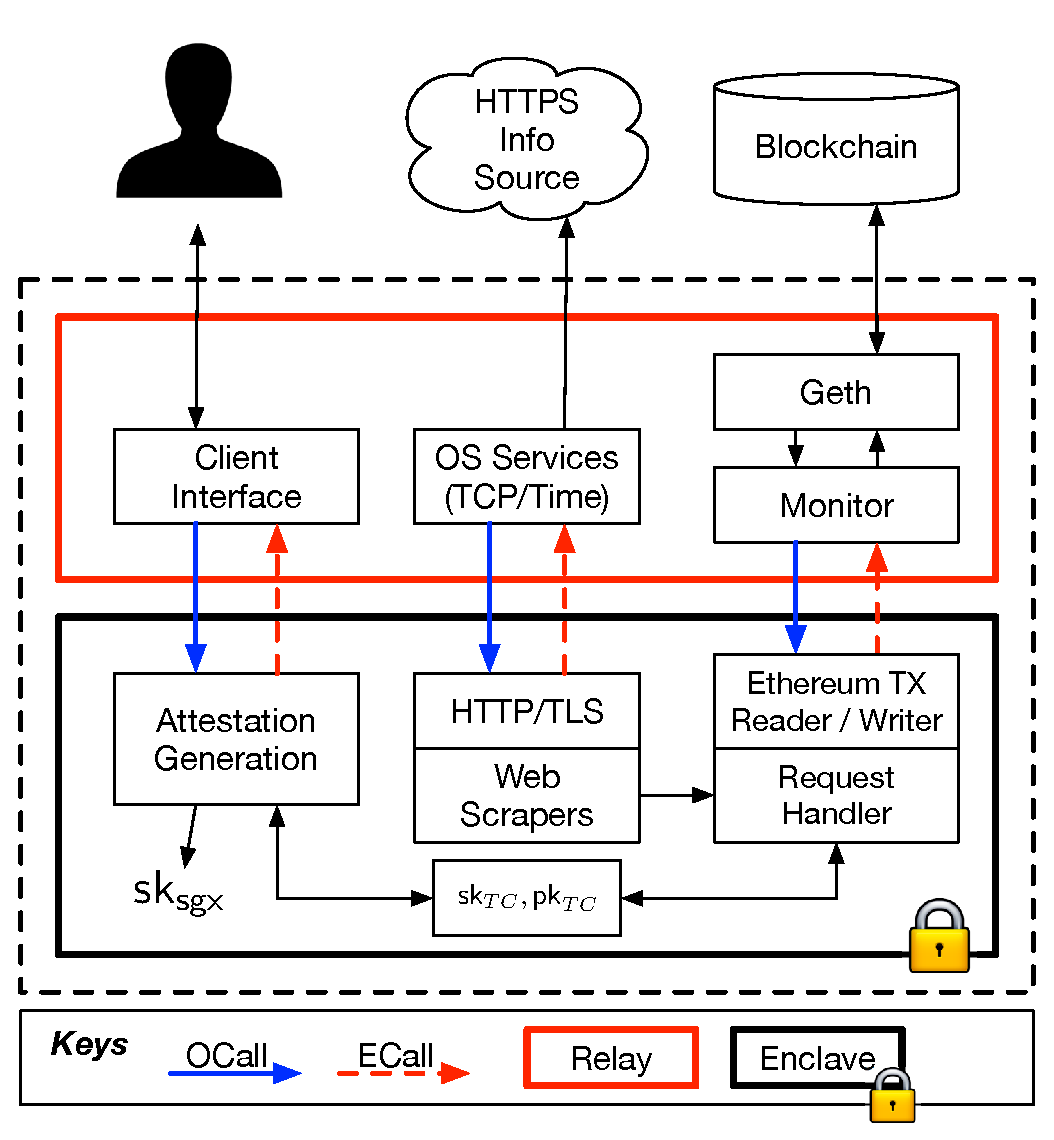
\includegraphics[width=0.45\textwidth]{figures/impl}

\begin{tikzpicture}
  [box/.style={entity, text width=1.5cm, inner sep=5pt},
   untrusted/.style={fill=red!33},
   double/.style={rectangle split, rectangle split parts=2},
   ecall/.style={color=blue,thick},
   ocall/.style={color=red!80!black,thick}]
  \matrix (m) [row sep=1.2em, column sep=0.6em]{
    \node[inner sep=0pt,anchor=south] (user) {
\includegraphics[width=1cm]{figures/user.eps}}; &
    \node[inner sep=0pt,draw,cloud,aspect=2.0,align=center,anchor=south](cloud) {\footnotesize HTTPS \\ websites}; &
    \node[box, cylinder, shape border rotate=90, aspect=.2,anchor=south](bc){blockchain};  \\[0.9em]

    \node[box,fill=white] (client) {Client \\ Interface}; & 
    \node[box,fill=white] (net) {TCP}; & 
    \node[box,fill=white,double,text width=2cm] (monitor) {\texttt{geth} \nodepart{second}{Blockchain \\ Interface}}; \\[0.6em]

    \node[box] (att) {Attestation \\ Generation}; &
    \node[box,double] (https) {HTTPS \nodepart{second}{Web \\ Scrapers}}; &
    \node[box,double,text width=2cm,] (req h){Ethereum TX \\ Reader/Writer \nodepart{second}{Request Handler}}; \\

    & \node[box,text width=2cm] (keys) {\pkTC, \skTC}; & \\
  };
  \node[anchor=west] (sk) at (keys.west-|att.west) {\skM};

  \draw[<->,thick] (user) -- (client);
  \draw[<->,thick] (net) -- (cloud);
  \draw[<->,thick] (monitor) -- (bc);

  \draw[->,ocall,transform canvas={xshift=-2mm}] (https) to (net);
  \draw[->,ocall,dashed,transform canvas={xshift=+2mm}] (net) to (https);

  \draw[->,ecall,transform canvas={xshift=-2mm}] (client) -- (att);
  \draw[<-,ecall,dashed,transform canvas={xshift=+2mm}] (client) -- (att);

  \draw[->,ecall,transform canvas={xshift=-2mm}] (monitor) -- (req h);
  \draw[<-,ecall,dashed,transform canvas={xshift=+2mm}] (monitor) -- (req h);

  \draw[<->,thick] (https.two east) -- (https.two east -| req h.two west);

  \draw[->,thick] (req h.south) |- (keys.east);
  \draw[->,thick] ([xshift=1.25em]att.south)  |- (keys.west);
  \draw[->,thick] (att.south-|sk.north) -- (sk);

  \begin{pgfonlayer}{background}
    \node [bg-box, inner sep=1.2em, tc-server-color, fit=(client)(monitor)(keys)] {};
    \node [inner sep=0.6em, untrusted, fit=(client) (net) (monitor)] {};
    \node [inner sep=0.6em, trusted, fit=(att) (https) (req h) (keys)] {};
  \end{pgfonlayer}

    \matrix (legend) [below=1.2em of m, matrix of nodes, column sep=0.75em, align=center]
  {
    \node[inner xsep=0] {\small \bf Legend:}; &
    \node[untrusted] (relay-leg) {\small Relay\vphantom{Ry}}; &
    \node[trusted] (enc-leg) {\small Enclave\vphantom{Ry}}; &
    \node[tc-server-color,rounded corners,text width=2.5em] (server-leg) {\small Server\vphantom{Ry}}; &
    \node[text width=1.75em] (ecall-leg) {}; &
    \node[text width=1.75em] (ocall-leg) {}; \\
  };

  \path[->,ecall,above] (ecall-leg.west) edge node {\small ecall} (ecall-leg.east);
  \path[<-,ecall,dashed,transform canvas={yshift=-0.4em}] (ecall-leg.west) edge (ecall-leg.east);

  \path[->,ocall,above] (ocall-leg.west) edge node {\small ocall} (ocall-leg.east);
  \path[<-,ocall,dashed,transform canvas={yshift=-0.4em}] (ocall-leg.west) edge (ocall-leg.east);
\end{tikzpicture}
\caption{Components of \tc Server}
\label{fig:tcserver_impl}
\end{figure}

For \tc, we recall that Fig.~\ref{fig:engineprotocol} shows the \encname code
$\engine$. Fig.~\ref{fig:relayprotocol} specifies the operation of the \medname,
the untrusted code in \tc, which we emphasize again provides essentially only
network functionality. We now give details on the services in the \encname and
the \medname and describe their interaction, as summarized in
Fig.~\ref{fig:tcserver_impl}.

\paragraph{\bf The \encname.} There are three components to the enclave code
\engine: An HTTPS service, Web Scrapers, which interact with data sources, and a
Request Handler, which services datagram requests. 

\vspace{2mm}

\noindent\emph{HTTPS Service.} We recall that the enclave does not have direct
access to host network functionality. \tc thus partitions HTTPS into a trusted
layer, consisting of HTTP and TLS code, and an untrusted layer that provides
low-layer network service, specifically TCP.  This arrangement allows the
enclave to establish a secure channel with a web server: The enclave itself
performs the TLS handshake with a target server and performs all cryptographic
operations internally, while the untrusted process acts as a network interface
only. We ported a TLS library (mbedTLS) into the SGX environment, as well as
HTTP code, which we minimized to meet the web-scraping requirements of \tc while
keeping the TCB small. To verify certificates presented by remote servers, we
hardcoded a collection of root CA certificates into the enclave code; in the
first version of \tc, the root CAs are identical to those in Chrome~\cite{}. By using its internal, trusted wall-clock time, it is possible to verify that a certificate has not expired. (We briefly discuss revocation in Appendix~\ref{sec:future}.)

\vspace{2mm}

\noindent\emph{Web Scrapers.} We implemented scrapers for our examples in Section~\ref{sec:applications} in an ad hoc manner for our initial implementation of \tc, and defer more principled, robust approaches to future work. 

\vspace{2mm}

\noindent\emph{Request Handler.} The Request Handler has two jobs: (1) Ingesting
a datagram request by parsing it in the serialization format specified by
Ethereum, decrypting it (if it's a private-datagram request), and dispatching
its parameters to the right scraper; and (2) Returning the response to the
request by generating an Ethereum transaction containing the requested datagram
(and parameters), serializing it as a blockchain transaction, and signing it
using \skTC. We implemented the Ethereum ABI and RLP, which respectively specify
the serialization of arguments and transactions in Ethereum. 

\vspace{2mm}

\noindent\emph{Attestation Generation.} Recall in Section \ref{sec:background}
we mentioned that an \emph{attestation} is an \emph{report} digitally signed by
the Intel-provided Quoting Enclave (QE).  Therefore two phases are involved in
generating \att. First, the \encname calls \texttt{sgx\_create\_report} to
generate a report with QE as the target enclave. Then the \medname forwards the
report to QE and calls \texttt{sgx\_get\_quote} to get a signed version of the
report, namely an attestation.

\paragraph{The \medname.} The \medname encompasses three components: A Client Interface, which serves attestations and timestamps, OS services, including networking and time services, and a Blockchain Interface. 

\vspace{2mm}

\noindent\emph{Client Interface.} As described in Section \ref{sec:architecture},
a client starts using \tc by requesting and verifying an attestation \att and checking the correctness of the clock in the \tc enclave using a fresh timestamp.
The Client Interface caches \att upon initialization of \engine. When it receives a web request from a client for an attestation,
it issues an ecall to the enclave to obtain a
Unix timestamp signed using \skTC, which it returns to the client along with \att. The client verify \att 
using the Intel Attestation Service (IAS)~\cite{} and then verify the timestamp using $\pkTC$ and check it using any trustworthy time service. 

\vspace{2mm}

\noindent\emph{OS services.} The \encname relies on the \medname to access networking and 
wall-clock time provided by the OS and implemented as ocalls.

\vspace{2mm}

\noindent\emph{Blockchain Interface.} The \medname's Blockchain Interface monitors the
blockchain for incoming requests and places transactions on the blockchain in order to
deliver datagrams. The Blockchain Interface incorporates an 
official Ethereum client, Geth~\cite{geth}. This Geth client can be configured with a JSON RPC server.  
The \medname  communicates with the blockchain indirectly via RPC calls to this server. For example, to insert a signed transaction, the \medname simply calls
\texttt{eth\_sendRawTransaction} with the byte array of the serialized
transaction. We emphasize that as the enclave holds \skTC, transactions are signed within the enclave.


\section{Security Analysis}
\label{sec:analysis}

Proofs of theorems in this section appear in Appendix~\ref{sec:analysis-proofs}.


\paragraph{Authenticity.}
Intuitively, authenticity means that an adversary (including a corrupt user, relay, or collusion thereof)
cannot convince \tcont to accept a datagram that differs from the expected content obtained by crawling the specified \weburl at the specified time.
In our formal definition, we assume that the user and \tcont behave honestly.
Recall that the user must verify upfront the attestation $\sigatt$ that vouches for the enclave's public key $\pksgx$.

\begin{definition}[Authenticity of Data Feed]
We say that the \tc protocol satisfies \emph{authenticity of data feed} if,
for any polynomial-time adversary that can interact arbitrarily with $\fsgx$,
it cannot persuade an honst verifier to accept $(\pksgx, \sigatt, \dgform:=(\weburl, \pkurl, T), \dgm, \sigma)$
where $\dgm$ is not the contents of $\weburl$ with the public key $\pkurl$ at time $T$.
More formally, for any probabilistic polynomial-time adversary $\algA$,
\[
\begin{array}{l}
\Pr\left[
\begin{array}{l}
(\pksgx, \sigatt, {\sf id}, {\sf params}, {\sf data}, \sigma) \leftarrow 
\algA^{\fsgx}(1^\lambda) :\\
\quad \left(\sigsgx.{\sf Verify}(\pkM, \sigatt, (\enclaveprog, \pksgx)) = 1\right) \wedge \\
\quad \left(\Sigma.{\sf Verify}(\pksgx, {\sf id}, {\sf params}, {\sf data})  = 1\right) \wedge\\
\quad {\sf data} \neq \enclaveprog({\sf params}) 
\end{array}
\right] \\[3pt] 
\leq {\sf negl}(\lambda)
\end{array}
\]
\label{defn:auth}
\end{definition}


\begin{theorem}[Authenticity]
Assume that $\sigsgx$
and $\Sigma$ are secure signature schemes (recall
that we follow Shi et al. \elaine{cite} who show
how to abstractly  
model SGX's group signature as a regular signature
scheme under a manufacturer public key $\pkM$),
%and assume that the cryptographic protocol used to realize the secure channel
%with $\pkurl$ is secure;
then, the above 
protocol achieves authenticity of data feed by Definition~\ref{defn:auth}.
\end{theorem}




\paragraph{Fee Safety.}
Our protocol in Section~\ref{sec:gas-protocol} ensures that an honest \tcs will not run out of money
and that an honest requester will not pay excessive fees without receiving data.
These properties are encapsulated in the following theorems.

\begin{theorem}[Gas neutrality for Town Crier]
If the \tc~\medname is honest,
Town Crier's wallet $\tcadd$ will have at least $\constgasmax$ remaining after each {\bf Deliver} call.
\end{theorem}


\begin{theorem}[Fair Expenditure for Honest Requester]
For any request $(\dgform, \dgcallback, \fee)$ submitted by an honest user $\reqcont$,
at most $\constgascancel$ of the user's total payment will not be spent on computation requested by and executed on behalf of that user.
\end{theorem}





\subsection{Other security concerns}
We treat side-channel attacks as outside the scope of our initial \tc architecture. Such attacks would be of particular concern should the \medname be compromised. Intel explicitly disclaims protections against side-channel attacks in SGX. The ability for the OS to monitor page faults incurred by a process running in an enclave is an example shown to be potentially serious in practice~\cite{}. Additionally, the \medname or any network adversary can potentially perform traffic analysis to determine what content the \encname is retrieving from a remote server~\cite{}, a potential threat to the confidentiality of private datagrams.



\elaine{TODO: we might want to add a discussion about
how Town Crier handles website updates. if the website
format is updated later -- which cannot be anticipated,
Town Crier should abort rather than sending false data feeds.} 



\section{Applications: Requesting Contracts}
\label{sec:applications}

We built and implemented several showcase applications which we plan
to launch together with Town Crier.
We give a description of these applications in this section,
and show experimental results in Section~\ref{sec:experiments}.
We refer the reader to Appendix~\ref{sec:applicationsfull}
for more details on these applicatins,
as well as $\reqcont$ code samples that demontrate
first-hand experience of how to use Town Crier's service.


\paragraph{Financial derivative ({\sf CashSettledPut}).}
Financial derivatives are among the most commonly cited smart contract
applications,
and exemplify the need for a data feed on financial instruments.
We implemented an example contract {\sf CashSettledPut} for a {\em cash-settled put option}.
This is an agreement for one party to buy an asset from the other at an agreed upon price on or before a particular date.
It is ``cash-settled'' in that the sale is implicit, i.e. no asset changes hands, only cash reflecting the asset's value.
%In our implementation, the issuer of the option specifies a strike price $P_S$, expiration date, unit price $P_U$, and maximum number of units $M$ she is willing to sell.
%A customer may send a request to the contract specifying the number $X$ of option units to be purchased and containing the associated fee ($X \cdot P_U$).
%A customer may then exercise the option by sending another request prior to the expiration date.
%{\sf CashSettledPut} calls \tc to retrieve the closing price $P_C$ of the underlying instrument on the day the option was exercised, and pays the customer $X \cdot (P_S - P_C)$.
%To ensure sufficient funding to pay out, the contract must be endowed with ether value at least $M \cdot P_S$.
%
\iffalse
\paragraph{Financial Derivatives.}  In order to implement a financial derivative as a smart contract, we require information about the corresponding financial instrument upon which the derivative depends (typically a stock).  As an example, we implemented a cash-settled put option.  The issuer of the option creates a contract for a particular stock, strike price, time period, unit price, and the maximum number of units he is willing to sell.  Customers may purchase the option by sending requests to the contract along with the associated fee indicating the number of units of the option they would like to buy.  Until the expiration date, customers may choose to exercise the put option by making another request to the option contract.  The contract then requests that TC retrieve the closing price of the underlying instrument on the day the option was exercised, and pays out to the customer the difference between the strike price and the closing price for each unit of the option purchased.  To ensure the contract always has sufficient funds to pay out, it must control value of at least the strike price times the maximum number of units sold.
\fi

\paragraph{Flight insurance ({\sf FlightIns}).}
Flight insurance indemnifies a purchaser should her flight be delayed or canceled.
We have implemented a simple flight insurance contract called {\sf FlightIns}.
Our implementation showcases \tc's {\it private-datagram} feature to address an obvious concern:
customers may not wish to reveal their travel plans publicly on the blockchain. 
Roughly speaking, 
a customer submits to $\tcont$ a 
request ${\sf Enc}_{\pkTC}({\sf req})$ 
encrypted under Town Crier enclave's public 
key $\pkTC$. The enclave decrypts
the request and checks its well-formedness (e.g., the request is submitted
sufficiently long before the flight time).
If well-formed, the enclave will fetch the flight information website
at a specified later time, and send to $\tcont$ a datagram indicating
whether the flight is cancelled. 
Finally, to avoid leaking information through timing (e.g.,
when the flight 
information website is accessed), random delays can be introduced to mitigate
the information leakage. 

%An insurer stands up {\sf FlightIns} with a specified policy fee, payout, and lead time $\Delta T$. ($\Delta T$ is set large enough to ensure that a customer can't anticipate flight cancellation or delay due to weather, etc.) To purchase a policy, a customer sends the {\sf FlightIns} a ciphertext  $C$ under the \tc's pubic key $\pkTC$ of the ICAO flight number $FN$ and scheduled time of departure $T_D$ for her flight, along with the policy fee. {\sf FlightIns} sends \tc a private-datagram request containing the current time $T$ and the ciphertext $C$. \tc decrypts $C$ and checks that the lead time meets the policy requirement, i.e., that $T_D - T \geq \Delta T$. \tc then scrapes a flight information data source several hours after $T_D$ to check the flight status, and returns to {\sf FlightIns} predicates on whether the lead time was valid and whether the flight has been delayed or cancelled. If both predicates are true, then {\sf FlightIns} returns the payout to the customer. Note that $FN$ is never exposed in the clear.

%Despite the use of private datagrams, {\sf FlightIns} as described here still poses a privacy risk, as the {\em timing} of the predicate delivery by \tc leaks information about $T_D$, which may be sensitive information; this, and the fact that the payout is publicly visible, could also indirectly reveal $FN$. {\sf FlightIns} addresses this issue by including in the private datagram request another parameter $t > T_D$ specifying the time at which predicates should be returned. By randomizing $t$ and making $t - T_D$ sufficiently large, {\sf FlightIns} can substantially reduce the leakage of timing information. 

\paragraph{Steam Marketplace ({\sf SteamTrade}).} 
Authenticated data feeds and smart contracts can enable
fair exchange of digital goods 
%(e.g., virtual items in games)
between Internet users who do not have pre-established trust.
To do this, we have developed an example application supporting
fair trade of virtual items for the Steam~\cite{steam},
an onling gaming platform that supports thousands of games and maintains its own marketplace, where users can trade, buy, and sell games and other virtual items.  
We implement a contract for the sale of games and items for ether that showcases \tc's support for {\it custom datagrams} through the use of Steam's access-controlled API.
In our implementation, 
the buyer sends ${\sf Enc}_{\pkTC}(\text{account credentials}, {\sf req})$
to $\tcont$,
such that Town Crier's enclave can log in as the buyer  
and determine from the web-page whether the virtual item
has been shipped.


%A user intending to sell items creates a contract {\sf SteamTrade} with his Steam account number $ID_S$, a list $L$ of items for sale and a price in ether for each.  In order to purchase some subset $L_B$ of the items, a buyer first uses a Steam client to create a trade offer requesting each item $i \in L_B$.  The buyer then submits to {\sf SteamTrade} a ciphertext $C$ under the \tc's public key $\pkTC$ of his Steam API key $K_S$, his account number $ID_B$, the list of items $L_B$, and a time period $T_B$ indicating how long the seller has to respond to the offer, along with an amount of ether equivalent to the sum of the specified prices of all items in $L_B$.  {\sf SteamTrade} sends \tc a custom datagram request containing the current time $T$, the account number $ID_S$, and the ciphertext $C$.  \tc decrypts $C$, delays for time $T_B$, then retrieves all trades between the two accounts identified by $ID_S$ and $ID_B$ within that time period by using the provided API key $K_S$.  \tc verifies whether or not a trade exactly matching the items in $L_B$ successfully occurred between the two accounts and returns the result to {\sf SteamTrade}.  If such a trade occurred, {\sf SteamTrade} sends the buyer's ether to the seller's account.  Otherwise the buyer's ether is refunded.

\iffalse
\paragraph{Steam Marketplace.} Steam \kyle{reference?} is an online gaming platform that supports thousands of games and maintains its own marketplace, where users can trade, buy, and sell games and other virtual items.  Through the Steam trading API, for which a key is issued to each user, we can construct a contract that implements the sale of games and items for ether using custom datagrams.  A user wishing to sell items creates a contract specifying the items to be sold along with a price in ether for each.  A user wishing to buy the items creates a Steam trade offer requesting the items (which the seller must accept out of band through either a Steam client or the Steam API), and then submits an Ethereum transaction with value in ether equal to the specified price along with an attached ciphertext containing a reference to the trade offer and his Steam API key.  The API key of either the buyer or the seller is required in order to view the contents of the trade.  The contract submits a request to TC using the provided ciphertext, and relies on TC to verify the contents and status of the trade and return the result.  If the trade was successfully accepted by the seller and the items transferred to the buyer, then the contract transfers the buyer's ether to the seller's account.  Otherwise if the trade is unsuccessful, the buyer's ether is refunded by the contract.

There is a clear parallel between the exchange of virtual goods for ether and the exchange of fiat currency for ether.  The contract remains mostly the same; virtual goods are simply replaced with dollars and the Steam API is substituted out for a (preferably read-only) API for a user's bank statements.  In both cases, the \encname must be trusted not to compromise the user's privacy (or worse if the provided API keys have additional privileges) when given access to their account statements.
\fi
%Discuss flight insurance as an example: We'd like to conceal the flight number and date. We might also want to conceal payment, so TC might ingest encrypted addresses and mix them internally.

%Micro-loans too? Linkage to Facebook / Keybase.io


\section{Future Work}
\label{sec:future}

We plan to develop \tc after its initial deployment and expect it to evolve to incorporate a number of additional features. These fall into two categories: (1) Expanding the security model to address threats outside the scope of the initial version and (2) Extending the functionality of \tc. Here we briefly discuss a few of these extensions.

\subsection{Expanding \tc threat model}

\begin{itemize}
\item{\em Freeloading protection.} Serious concerns have  arisen in the Ethereum community about ``parasite contracts'' that forward or resell datagrams---particularly those from fee-based data feeds~\cite{parasite}. We plan to deploy a novel mechanism in \tc to address this concern. Suppose contract \reqcont involves a set of parties / users $U = \{U_i\}_{i=1}^n$. Each player $U_i$ generates an individual share $(\sk_i, \pk_i)$ of a global keypair $(\pk, \sk)$, where $\sk = \sum_{i=1} \sk_i$ and $\pk = \prod_{i=1} \pk_i$, and communicates a ciphertext $E_{\pkTC}[\sk_i]$ to \tcont, e.g., by including it in a datagram request. Players then jointly set  up under public key $\pk$ a wallet $\specialwallet$ for datagram transmission by \tcont. 

Thanks to the homomorphic properties of ECDSA, \tcont can compute $\sk$ (non-interactively) and send datagrams from $\specialwallet$. But the users $U$ collaboratively \emph{can also compute $\sk$ and send messages from $\specialwallet$}. Consequently, while each user $U_i$ can individually be assured that a datagram sent to \reqcont by \tcont from $\specialwallet$ is valid (as $P[i]$ didn't collude in its creation), other players cannot determine whether a datagram was produced by $\tcont$ or $U$, and thus whether or not it is valid. Such a \emph{source-equivocal datagram} renders data from parasite contracts less trustworthy and thus less attractive. 
\item{\em Traffic-analysis protection.} As noted in the body of the paper, \medname can observe the pattern of data sources accesses made by \tc. By correlating with activity in \tcont, an adversarial \medname can thus infer the data source targeted by private datagrams, as well as the timing---and potentially, based on traffic analysis, of the \encname's HTTPS requests. (See, e.g.,~\cite{chen2010side}.) In the example contract {\sf FlightIns} in Section~\ref{sec:applications}, this issue is partially addressed through the insertion of random delays into \tc responses. We intend to develop a comprehensive approach to mitigating traffic analysis in \tc. This approach will include, for the problem of traffic analysis of web scraping, the incorporation of facilities in the \encname to make chaff or decoy data requests, i.e., false requests, to both the true data source and well as non-target data sources. 

\item{\em Revocation support.} Revocation of two forms can impact the \tc service. 

First, the certificates of data sources may be revoked. To address this issue, given its ability to establish external HTTPS connections, \tc could easily make use of Online Certificate Status Protocol (OCSP) certificate checking. This functionality would amount to an additional form of web scraping, and could be executed in parallel with web scraping to support datagram requests, resulting in minimal additional latency.

Second, an SGX host could become compromised, prompting revocation of its EPID signatures by Intel. The Intel Attestation Service (IAS) will reportedly provide support for online attestation verification and thus for revocation. Conveniently, clients use the IAS when checking the attestation $\sigatt$, so no modification to \tc is required to support the service.


\item{\em SLAs.} Were \tc to be deployed as a fee-for-service system, requesters might wish to see Service Level Agreements (SLAs) enforced. A temporary outage on a \tc host or a malicious \medname could cause a delay in datagram delivery, potentially with aftereffects in relying contracts. An SLA could be implemented as an indemnity paid to a contract if a datagram is not delivered within a specified period of time. This feature could itself be implemented, for example, as an entry point in $\tcont$. (Naturally care would be required to ensure that $\tcont$ holds funds sufficient for payout in the case of a general delivery failure.)

\item{\em Hedging against SGX compromise.} We discussed in Section~\ref{subsec:enhanced_robustness} and demonstrated in Section~\ref{subsec:hedging} how \tc can support majority voting across SGX hosts and/or data sources to hedge against failures in either (outside \tc's basic security model) via majority voting. It would be possible to reduce the latency and gas costs of such voting with design enhancements to \tc. Specifically, for the case of SGX voting, we plan to investigate a scheme in which consensus on a datagram value $X$ is reached off-chain among SGX-enable \tc hosts  via Byzantine consensus. These hosts may then use a threshold digital signature scheme to sign the datagram response from ${\cal W}_{TC}$. To ensure that the response is delivered to the blockchain, each participating host can monitor the blockchain and itself transmit the response in the case of an observed delivery failure. This approach will largely eliminate the incremental gas cost of majority voting across SGX instances.

\end{itemize}

\subsection{Expanding \tc functionality}

\begin{itemize}
\item{\em New opcodes.} Ethereum's developers~\cite{Buterinpersonal} have indicated an intention to expand the range of supported cryptographic primitives in Ethereum and stated that they are amenable to the authors' suggestion of incorporating opcodes supporting Intel's EPID in particular, which would enable efficient attestation verification within the blockchain. 
\item{\em Migration to data-source feeds.} Ultimately, we envision that data sources may wish themselves to serve as authenticated data feeds. To do so, they could simply stand up \tc as a front end. As a first step along this path, however, an independent \tc service might provide support for XML-labelled data from data sources, enabling more accurate and direct scraping and intentional identification of what data should be served. We plan to build support for such explicit data labeling into \tc should this approach prove attractive to data sources.
\item{\em Generalized custom datagrams.} In our example smart contract {\sf SteamTrade}, we demonstrated a custom datagram that is essentially hardwired: It employs a user's credentials to scrape her individual online account. A more general approach would be to allow contract owners to specify their own generalized functionalities--scrapers and/or confidential contract modules---as general purpose code, achieving a data-source-enriched emulation of private contracts as in Hawk~\cite{hawk}, but with much lower resource requirements. Furnishing large custom datagrams on the blockchain would be prohibitively expensive, but off-chain loading of code would be quite feasible. Of course, many security and confidentiality considerations arise in a system that allows users to deploy arbitrary code, giving rise to programming language challenges that deployment of this feature in \tc would need to address.
\end{itemize}



\section{Conclusion}
\label{sec:conclude}

We have introduced \tcs (\tc), an authenticated data feed for smart contracts specifically designed to support Ethereum.
Use of Intel's new SGX trusted hardware allows \tc to serve datagrams with a high degree of trustworthiness.
We defined \emph{gas sustainability}, a critical availability property of Ethereum services,
and provided techniques for shrinking the size of a hybrid TCB spanning the blockchain and an SGX.
We proved in a formal model that \tc serves only data from authentic sources,
and showed that \tc is gas sustainable and minimizes cost to honest users should the code behave maliciously.
In experiments involving end-to-end use of the system with the Ethereum blockchain, we demonstrated \tc's practicality, cost effectiveness, and flexibility for three example applications.
We believe that \tc offers a powerful, practical means to address the lack of trustworthy data feeds hampering Ethereum evolution today and that it will support a rich range of applications.
Pending deployment of the Intel Attestation Service (IAS), we will make a version of \tc freely available as a public service.


\pagebreak
\appendix 

OLD MATERIAL

\section{Introduction}

\section{Identifying Client Contracts}
The Authenticated Data Feed (ADF) needs some method to identify and serve prospective clients.  There are two on-chain methods: registration and client flags.  The registration method requires an additional transaction and will therefore incur an additional fee.  The flags method must scan all contracts at every block update to support dynamic data requests.  It may therefore be useful to support both methods, using the blockchain crawler for one-time requests and registration for more complicated contracts, depending on the resource costs of the crawler.
\subsection{Registration / Explicit Requests for Data}
	This requires the client to initiate communication to the ADF with a \emph{Initial Client Request} message, which consists of a (potentially zero-value) transaction to the ADF address with a message specifying what signed data it wants. 
	
\subsection{Client Flags / ADF Blockchain Crawler}
	This method requires only that the client contract has in its key/value store a flag indicating its request for service from the ADF and the specifics of the data it wants.  The ADF can then crawl the blockchain looking for contracts with this specific flag set and read the data requested.
	
\subsection{Off Chain Communication}
	The ADF may be notified of prospective clients by any manner of off-chain communication however there will be no public record of this request.  The ADF may then selectively deny service.  Malicious clients may also have an easier time flooding the ADF with requests, compared to the other two methods which have an Ether cost (contract creation).\\

\subsection{Migration Path}

Ultimately, we expect sources themselves to act as ADFs. The migration path is : (1) Town Crier; (2) XML labels on data; (3) Integration of Town Crier features into source directly

\section{Payment Methods}	
\subsection{Separate Fair Exchange Contracts}
    The ADF or the client contract creates or uses an existing \emph{fair exchange contract} for each data request.  This contract requires input from the client in the form of some amount of Ether (this can happen during the creation of the contract), and the signed data from the ADF.  Once both inputs have been received, the contract sends the Ether to the ADF and the data to the client. Note the client should send the currency first as once the ADF publishes the signed data it will be publicly visible (unless we use zero-knowledge proofs). If the ADF fails to deliver the data within a time period then the client's money is refunded.\\
    \indent The main benefit of this method is that the fair exchange contract should be easier to verify for both parties.  Depending on the specifics of the attestation it needs to check, it may be possible for the contracts to be completely templated.  Also note that creating a new contract will incur a transaction fee.  These data fair exchange contracts can potentially batch data requests and verification and can be re-used for subsequent requests if desired. \fan{the client and the ADF should agree on the content of this contract. In my mind this template could be provided by an ADF service provider along with other information on their website. For example, clients can browse ADF's website for pricing info, the public address, an template for generating request and ensuring fair exchange and the public key. Then clients can embed these information in there own contract.}\\
    \kyle{This is my thought as well.  A client may extract the address, pricing info, and a code template for fair exchange from the ADF website.  The issue I was trying to get at was that verifying the bytecode of one function in a contract may be more difficult than simply verifying an entire contract's bytecode due to having to isolate the function.  I don't know whether isolating a function is hard or if the bytecode may change depending on the client contract (offsets, compilers, etc), but at the very least it involves the extra step of checking the function entry point in addition to simply matching the hash of the bytecode}
    
\subsection{Payment Built-in to the Client Contract}
    The client contract includes a function that accepts signed data and pays out the specified amount of coins to the sender if the data is correct.  This requires the ADF to verify the correctness of the function and that the client has sufficient funds.  It would be potentially useful for this function to be templated for ease of use and verification, and at the very least it needs to conform to some specification agreed upon by the client and ADF. 
    
\subsection{Payment built-in to the ADF}
    The client may send payment directly to an ADF contract as part of its initial request.  The ADF contract code must maintain a list of clients and their corresponding requests.  It must also verify the attestation on the data before forwarding it to the client since it has already been paid.  The client must verify that the ADF contract code is correct.
    
\fan{Do all of 9 combinations of (2.1, 2.2, 2.3) and (3.1, 3.2, 3.3) make sense? Or we should point out the best combinations?}
\kyle{All combinations make sense to me with the exception of client flags and payment built-in to the ADF (2.2, 3.3)}
    
\section{Privacy}
Everything posted to the blockchain is publicly visible, including all data requests directed towards the ADF.  It is possible to encrypt data requests, as the ADF may decrypt and process them off-chain.  It is not always possible to encrypt the responses, as the contract requesting the data will often need to process the data.

\subsection{Privacy From Peers}
    In some cases clients may want to keep their requests for data private.  For example a client requesting information about the weather may need to provide his zip code for accurate local results.  However he may not wish for his zip code to be publicly visible.  To solve this, he may encrypt his zip code (or his entire request) with the ADF's public key before posting it to the blockchain.  Note that all encryption and decryption operations can be done off-chain to avoid incurring excessive gas fees.\\

\subsection{Partial Privacy From ADFs}
    Clients may also wish to keep some information private from the ADF.  Consider again a client requesting information about the weather who wishes to keep his zip code private not only from the public, but from the ADF as well.  This can be accomplished by utilizing two ADFs $A_1$ and $A_2$.  The client creates $n-1$ randomized decoy requests for data along with his actual request.  He orders these requests such that his actual request appears at a randomly chosen index $i$.  He then encrypts all requests under the public key of $A_1$ and submits all $n$ encryptions in order to $A_1$.  He encrypts $i$ under the public key of $A_2$ and submits the encryption to $A_2$.  $A_1$ decrypts and computes the results for all $n$ queries and submits the results to $A_2$.  $A_2$ returns to the client the $i$th result.  So long as the two ADFs do not collude (in the context of the weather example, this means neither ADF can know both the zip codes and the index $i$), $A_1$ can only guess the clients true data with probability $\frac{1}{n}$.  \kyle{There is definitely some leakage here if the response returned by $A_2$ is in plaintext} 
    
    
    \kyle{The issue is that the information has to appear in plaintext somewhere on the blockchain in order for a contract to use it, otherwise $A_2$ could simply encrypt the response under the public key of the client.  We could obfuscate the result with a mask, but the client contract will still need to unmask the data to use it, and when it does anyone can read it.  Then in our example $A_1$ knows what the weather was at the clients zipcode and may cross reference with the zipcodes he was given}
    \ari{As regards leakage, that's right. If the output of the contract depends on the zip code, information will leak}
    \ari{Remember the compression trick as well. Let $G$ be an additive group over 5-decimal-digit numbers. Let $PRF_k: \{0,1\}^{*} \rightarrow G$ be a PRF. To send a correct zip code $z$ in list of $n$ zip codes, of which $n-1$ are ``decoys'', the client selects a key $k$ and index $i \in [1,n]$ at random. The client sends $(k,p = PRF_k[i] - z)$. The ADF decodes the list as $\{PRF_k[1] - p, \ldots, PRF_k[n]  - p\}$.}

\subsection{Fully Private Requests}
    If a client wishes to keep the entirety of the request private, he may do so by leveraging the ADF's trusted hardware.  The initial request is encrypted under a public key stored in the trusted hardware, which processes the request.  A malicious ADF operator may only determine the sources which are contacted as a result of the request, and if necessary these can be masked with decoy queries as well.

\subsection{Decoy Requests}
Decoy requests for partially private protocols should be in the same class as the real request.  In the weather example, all zipcodes provided as decoy requests should be experiencing the same weather as in the actual request.  As the outcome of the contract is public, the ADF will be able to determine the value of the weather at the client's zipcode and can discount all decoys that do not match.\\\\
If the class of decoy requests can be pseudorandomly generated, we can save data transmission fees by sending only a random function, a seed, and a mask to ensure that the real request is computed.

\section{Example: Travel Insurance}
An insurance company may provide insurance for canceled flights by maintaining an Ethereum contract on the blockchain.  The source code of this contract should be public to allow potential customers to verify its correctness.  A customer may then purchase insurance by paying a predetermined amount of ether into the contract.  In addition, this transaction should include identifying information (flight number) for the flight for which the customer wishes to be insured.  However, the customer may wish to hide the flight number in order to avoid publicly revealing which flight he/she will be on.  To achieve this, the customer may encrypt the flight number under a public key whose corresponding private key is stored only in the ADF's trusted hardware.  Thus only enclave code will be able to view the unencrypted flight number, preventing even a malicious ADF or data center operator from compromising privacy. Once the ADF is made aware of the requests (as detailed in section 2), it proceeds by decrypting the flight number and determining whether or not the relevant flight was canceled. It strips all identifying information from response, and returns either ``Canceled'' or ``Not canceled.''  

\section{Applications}


\begin{itemize}
\item micro-insurance:
    \begin{itemize}
    \item weather
    \item item delivery
    \item flight delay (note: something we could implement easily ourselves...)
    \end{itemize}
\item Ethereum and USD exchange
\item stock price
\item BTC exchange (with and without ADF)
\item Simple derivatives
\item sports betting
\end{itemize}







\section{Version 1}

Here we define and discuss proposed extensions to the Town Crier protocol.

\subsection{Request Cancellation}

In order to provide recourse if the system is compromised and disabled or datagrams are delayed beyond a reasonable time,
there can be a way to cancel requests for a refund.
The refund must withhold a fixed fee of $F_{\rm min}$ in order to ensure that malicious aborts cannot bankrupt the ADF, but the rest of the fee can be refunded at any time.
If the ADF attempts to deliver a datagram for a canceled request, it will simply receive the $F_{\rm min}$ needed to cover its gas costs for the attempted delivery and not deliver any data.

In order to safely handle request cancellations, we now have to store verification data on the blockchain itself.
This will be considerably more expensive, but the Ethereum protocol supports it cleanly.
For notational simplicity, we use four blockchain storage functions.
They functions create a map from integers to arbitrary data values in the domain $V$.
\begin{itemize}
  \item {${\sf store} : \mathbb{N} \times V \to \emptyset$.}
    This stores a key with an associated value in the map and returns nothing.

  \item {${\sf load} : \mathbb{N} \to V \cup \{\bot\}$.}
    This returns the value associated with the given key or $\bot$ if the key is not in the map.

  \item {${\sf storeContains} : \mathbb{N} \to \{0, 1\}$.}
    This returns whether or not the key exists in the map.

  \item {${\sf remove} : \mathbb{N} \to \emptyset$.}
    This removes the key and its associated value if it is in the map and otherwise does nothing.
\end{itemize}
Table~\ref{tbl:Ctc-with-cancellation} describes the new \tcont blockchain.
The rest of the protocol need to change (save for calls to Deliver requiring slightly different arguments).

\begin{table}[htb]
\begin{tabularx}{\linewidth}{|@{\hspace{3pt}}r@{\hspace{1ex}}X@{\hspace{3pt}}|}
  \hline

  \multicolumn{2}{|c|}{\tcont with Cancellation} \\ [1ex]
  {\bf Init:} & Set ${\sf reqs} := \emptyset$ and ${\sf reqCnt := 0}$ \\
  {\bf Request:} & Upon receiving $({\sf type}, {\sf callback}, \${\sf fee})$ from a user $\mathcal{P}$: \\
                 & If $(\${\sf fee} < F_{\rm min}$ or $\${\sf fee} > F_{\rm max})$ \\
                 & \hspace*{1em} Return with no effect. \\
                 & Set ${\sf reqID} := {\sf reqCnt}$. \\
                 & Set ${\sf reqCnt} := {\sf reqCnt} + 1$. \\
                 & ${\sf store}({\sf reqID} \mapsto (\mathcal{P}, \${\sf fee}))$. \\
                 & Return ${\sf reqID}$. \\
  {\bf Deliver:} & Upon receiving $({\sf reqID}, {\sf data}, {\sf callback})$ from a user $\mathcal{P}$: \\
                 & If $\mathcal{P} \neq \textrm{\sgxadd}$ \\
                 & \hspace*{1em} Return with no effect. \\
                 & If $!{\sf storeContains}({\sf reqID})$ \\
                 & \hspace*{1em} Send $F_{\rm min}$ to \sgxadd. \\
                 & \hspace*{1em} Return with no further effect. \\
                 & $(*, \${\sf fee}) \leftarrow {\sf load}({\sf reqID})$. \\
                 & Call ${\sf callback}({\sf data})$ providing $\${\sf fee} - F_{\rm min}$ ether as the maximum gas. \\
                 & Send $\${\sf fee}$ ether to \sgxadd. \\
                 & ${\sf remove}({\sf reqID})$. \\
  {\bf Cancel:}  & Upon receiving $({\sf reqID})$ from a user $\mathcal{P}$: \\
                 & If $!{\sf storeContains}({\sf reqID})$ \\
                 & \hspace*{1em} Return with no effect. \\
                 & $(\mathcal{R}, \${\sf fee}) \leftarrow {\sf load}({\sf reqID})$. \\
                 & If $\mathcal{P} \neq \mathcal{R}$ \\
                 & \hspace*{1em} Return with no effect. \\
                 & Send $\${\sf fee} - F_{\rm min}$ to $\mathcal{P}$. \\
                 & ${\sf remove}({\sf reqID})$. \\

  \hline
\end{tabularx}
\caption{Definition of the \tcont contract with cancellation.}
\label{tbl:Ctc-with-cancellation}
\end{table}

Using the same adversarial model, we can make the same guarantees of this new system as we did for the original Town Crier system.
Even if a malicious user cancels their request just as Deliver is being called, the cancellation fee is enough to reimburse \sgxadd for any gas costs.

If we expand the adversarial model to allow for arbitrary denial of service attacks against the Town Crier system (but not the blockchain),
the new Cancel functionality allows affected users to recover most of their fee with no action from the Town Crier system.


\subsection{Service-level Agreements}

We start by noting that a service-level agreement (SLA) is generally implemented by paying recompense if it is violated.
This seems extreme if the service is not run for a profit, so thus we will assume that the costs of any SLA payments are funded by profits gained when the SLA is not violated.
For Town Crier, these profits can be implemented by simply increasing $F_{\rm min}$ above the gas cost necessary to run Deliver.
In this case, the extra money will be profit.
Note that if this happens, the cancellation fee could remain simply enough to recoup gas costs and not include the profit.

In this system, and SLA could consist of a maximum amount of time before a datagram is delivered.
If the user wishes to cancel a request before that time, it would be considered a voluntary cancellation and incur a cancellation fee high enough to cover gas costs of an attempted delivery.
If, however, the SLA has expired before the request is canceled, then not only would a cancellation not incur a fee, the user would be returned their entire initial fee and an SLA-violation recompense.
This could be a small value that would be need to later be paid back by Town Crier system out of the profits from successfully-deliver requests in order to prevent the contract from going bankrupt.

This mechanism presents some danger if a large number of SLAs are violated at the same time and the Town Crier system is unable to provide enough funds to the contract to make all of the recompense payments.
In this case, there could be a lightweight function on the contract to inform a user whether or not there is sufficient funding to make an SLA payment.
This function could either before cancellation requests or it could be before a request is made.
The former case would attempt to guarantee that a cancellation request right now would include an SLA payment.
The latter would attempt to ensure that a new request would always have money set aside to pay for an SLA violation.
Both of these utility functions may be subject to a race condition of another user making a cancellation or new request between the utility call on the actual call, thus costing an honest user money.









\section{Basic Protocol}

\subsection{A Gas-Free Basic Protocol}
For simplicity, we first describe a gas-free version of our basic protocol.
This basic protocol improves the strawman solution 
by resolving the aforementioned two issues.

\paragraph{Enclave-specific keys.}
To avoid having to verify a group signature on the blockchain,  
during enclave initialization, 
we have each enclave generate its enclave-specific 
key pair denoted $(\pksgx, \sksgx)$.
The $\sksgx$ is retained within the enclave and used
to sign the datagrams extracted from data sources during the request phase.
Since Ethereum itself 
already verifies signatures on messages sent from users (i.e.,
users interact with the 
Ethereum blockchain through an authenticated channel), 
we devise a trick to {\it piggyback the signature 
verification on top of Ethereum's already existing signature verfication mechanism}.
This means that the SGX enclave must sign datagrams using the \elaine{fill in name}
signature scheme that is compatible with Ethereum's signature verification.
This way, we need not implement a separate signature verification
in the user-defined $\tcont$ contract.
This saves 
not only software engineering effort, but more importantly, gas.

To make this idea fully work, in an offline phase, 
a user must verify an SGX attestation vouching for its own enclave-specific 
public key  $\pksgx$.
This $\pksgx$ is hardcoded inside the blockchain contract $\tcont$. 
The user is responsible for making sure that this hardcoded $\pksgx$ has an 
appropriate SGX attestation before interacting with the $\tcont$ 
blockchain contract.

\paragraph{Instantiating trusted absolute clock.}
Since SGX's trusted clock provides only relative time with 
respect to a reference point, 
we will rely on 
the following mechanism to realize a trusted {\it absolute} clock. 
\begin{itemize}[leftmargin=5mm]
\item
{\bf Offline calibration.}
In an offline phase, a user $U$ performs the following calibration protocol
with the SGX enclave:

\elaine{this formal notation needs to be changed, it is not compatible
with other formal notation.}

\begin{tabular}{rl}
$\mathcal{U}$: & get absolute $T_0$ from a trusted source \\
$\mathcal{U}$: & pick random ${\sf nonce}$\\
$\mathcal{U} \rightarrow \fsgx$: & ${\sf nonce}$\\
$\fsgx \rightarrow \mathcal{U}$: & (${\sf clock\_ref}$, $\Delta T_0$, ${\sf nonce}$)\\
$\mathcal{U}$: & record ${\sf clock\_ref}$, $\Delta T_0$
\end{tabular}

\elaine{the above assumes that 
an authenticated channel has been established.}

\item
{\bf Online trusted absolute clock.}
Whenever $\fsgx$ gives the relative time $\Delta T$ with respect
to ${\sf clock\_ref}$, the user 
{\it i)} checks that ${\sf clock\_ref}$ agrees with the saved
reference point, and 
{\it ii)}
computes $T_0 + \Delta T - \Delta T_0$
as the absolute time.
\end{itemize}


\paragraph{Formal protocol description.}

\begin{figure}
\begin{boxedminipage}{\columnwidth}
\begin{center}
{\bf User: offline attestation of SGX enclave}
\end{center}
\begin{tabular}{l}
{\bf Inputs}: $\pkM$, $\pksgx$, $\enclaveprog$, $\sigatt$ \\[5pt]
{\bf Checks:} \\
Assert $\enclaveprog$ is the expected enclave code\\
Assert $\sigsgx.{\sf Verify}(\pkM, \sigatt, (\enclaveprog, \pksgx))$ \\
Assert \tcont is correct and parametrized w/ \pksgx\\
{\it //~now okay to rely on \tcont}
\end{tabular}
\end{boxedminipage}
\caption{A user checks the Town Crier blockchain contract \tcont, 
and verifies an SGX attestation of the enclave's code and its public key $\pksgx$ before 
entering a contract that calls \tcont.
\elaine{here we use a simplified abstraction, but the actual implementation
also involves verifying the revocation list.}
%\elaine{there is a notational mismatch here. here we write RL explicitly, but
%not in the Fsgx abstraction}
} 
\end{figure}


\begin{figure}
\begin{tabularx}{\linewidth}{|@{\hspace{3pt}}r@{\hspace{1ex}}X@{\hspace{3pt}}|}
  \hline

  \multicolumn{2}{|c|}{{\bf Town Crier blockchain contract \tcont}} \\ [1ex]
  {\bf Request:} & On recv $({\sf id}, {\sf params}, {\sf callback})$ from some $\reqcont$: \\
%                 & If $(\${\sf fee} < F_{\rm min}$ or $\${\sf fee} > F_{\rm max})$ \\
%                 & \hspace*{1em} Return $\${\sf fee}$ to $\pkU$ \\
                 & Record $({\sf id}, {\sf params}, {\sf callback})$ \\
  {\bf Deliver:} & On recv $({\sf id}, {\sf params}, {\sf data})$ from $\pksgx$: \\
		 & Let $({\sf id}, {\sf params'}, {\sf callback} )$ be the most recently recorded tuple for ${\sf id}$\\
		 & Assert ${\sf params} = {\sf params}'$\\
                 & Call ${\sf callback}({\sf data})$ \\
%                 & Send $\${\sf fee}$ ether to $\Psgx$. \\

  \hline
\end{tabularx}
\caption{
A simple, fee-free version of the Town Crier contract \tcont.
Note that communication 
with \tcont is through an authenticated channel implemented through digital signatures (which
are not explicitly expressed in our notation).
}
\label{tbl:tc-contract}
\end{figure}

\begin{figure}
\begin{boxedminipage}{\columnwidth}
\begin{center}
{\bf Town Crier's enclave program}
\end{center}
\begin{tabular}{l}
%{\bf Inputs}:  ${\sf params}$, \\[5pt]
{\bf Initialize}:  On receive ``initialize'': \\ %{\it //~called only once upfront}\\
\quad $(\pksgx, \sksgx) := \Sigma.{\sf KeyGen}(1^\lambda)$\\
\quad Record $(\pksgx, \sksgx)$\\
\quad Output $\pksgx$   {\it //~incl. in measurement \& attestation } 
\\[5pt]

{\bf Resume:} On receive $({\sf id}, {\sf params})$\\
\quad Parse ${\sf params} := (\weburl, \pkurl, T) $:\\
%\quad Parse ${\sf params} := (\weburl, \pkurl, T)$ \\
\quad $T_{\textrm{start}} := \clock()$\\
\quad Establish secure channel w/ $\weburl$ w/ public key $\pkurl$ \\
\quad Download the webpage at $\weburl$\\
\quad $T_{\textrm{end}}: = \clock()$\\
\quad Assert ${\sf round}(T_{\textrm{start}}) = {\sf round}(T_{\textrm{end}}) = T$\\
\quad Parse webpage and extract ${\sf data}$\\
\quad $\sigma := \Sigma.{\sf Sign}({\sksgx}, ({\sf id}, {\sf params}, {\sf data}))$\\
\quad Output $(({\sf id}, {\sf params}, {\sf data}), \sigma)$
\end{tabular}
\end{boxedminipage}
\caption{
SGX enclave's code.
} 
\end{figure}


\begin{figure}
\begin{boxedminipage}{\columnwidth}
\begin{center}
{\bf Town Crier's untrusted relay $\relay$}
\end{center}
\begin{tabular}{l}
{\bf Initialize}:\\
Send ``initialize'' to $\fsgx[\enclaveprog, \relay]$\\
On receive $(\pksgx, \sigatt)$ from $\fsgx[\enclaveprog, \relay]$:\\
\quad Publish $(\pksgx, \sigatt)$\\[5pt]

{\bf  Loop forever}: \\
When \tcont receives new request $({\sf id}, \_, {\sf params})$:\\
\quad Parse ${\sf params} := (\weburl, \pkurl, T)$\\
\quad Fork: \\
\ \quad Wait till time $T$\\
\ \quad Send $(\text{``resume''}, {\sf params})$ to $\fsgx[\enclaveprog, \relay]$ \\
\ \quad On recv $(({\sf id}, {\sf params}, {\sf data}), \sigma)$ from $\fsgx[\enclaveprog, \relay]$:\\ 
\ \quad \quad  {\sf AuthSend} $({\sf id}, {\sf params}, {\sf data})$ to \tcont
\end{tabular}
\end{boxedminipage}
\caption{Town Crier untrusted relay. For simplicity, here we assume that there is only 
a single enclave program. When multiple data feed sources 
are supported, 
we need multiple enclaves that instantiate different parsers for different sites.
In this case, the Town Crier relay also initialize all enclave instances
and route the request to the correct enclave instance.}
\end{figure}














\end{document}

